% !TeX spellcheck = en_US
%%%%%%%%%%%%%%%%%%%%%%%%%%%%%%%%%%%%%%%%%
% Masters/Doctoral Thesis 
% LaTeX Template
% Version 2.5 (27/8/17)
%
% This template was downloaded from:
% http://www.LaTeXTemplates.com
%
% Version 2.x major modifications by:
% Vel (vel@latextemplates.com)
%
% This template is based on a template by:
% Steve Gunn (http://users.ecs.soton.ac.uk/srg/softwaretools/document/templates/)
% Sunil Patel (http://www.sunilpatel.co.uk/thesis-template/)
%
% Template license:
% CC BY-NC-SA 3.0 (http://creativecommons.org/licenses/by-nc-sa/3.0/)
%
%%%%%%%%%%%%%%%%%%%%%%%%%%%%%%%%%%%%%%%%%

%----------------------------------------------------------------------------------------
%	PACKAGES AND OTHER DOCUMENT CONFIGURATIONS
%----------------------------------------------------------------------------------------

\documentclass[
11pt, % The default document font size, options: 10pt, 11pt, 12pt
%oneside, % Two side (alternating margins) for binding by default, uncomment to switch to one side
english, % ngerman for German
onehalfspacing,
%singlespacing, % Single line spacing, alternatives: onehalfspacing or doublespacing
%draft, % Uncomment to enable draft mode (no pictures, no links, overfull hboxes indicated)
%nolistspacing, % If the document is onehalfspacing or doublespacing, uncomment this to set spacing in lists to single
%liststotoc, % Uncomment to add the list of figures/tables/etc to the table of contents
%toctotoc, % Uncomment to add the main table of contents to the table of contents
%parskip, % Uncomment to add space between paragraphs
%nohyperref, % Uncomment to not load the hyperref package
headsepline, % Uncomment to get a line under the header
%chapterinoneline, % Uncomment to place the chapter title next to the number on one line
%consistentlayout, % Uncomment to change the layout of the declaration, abstract and acknowledgements pages to match the default layout
]{theme} % The class file specifying the document structure

\usepackage[utf8]{inputenc} % Required for inputting international characters
\usepackage[T1]{fontenc} % Output font encoding for international characters

\usepackage{mathpazo} % Use the Palatino font by default

\usepackage[backend=bibtex, style=chem-acs, natbib=true]{biblatex}

\DeclareCiteCommand{\citeauthor}%
{\boolfalse{citetracker}%
	\boolfalse{pagetracker}%
	\usebibmacro{prenote}}
{\ifciteindex
	{\indexnames{labelname}}
	{}%
	\printtext[bibhyperref]{\printnames{labelname}}}
{\multicitedelim}
{\usebibmacro{postnote}}

\usepackage{subcaption}

\addbibresource{bibliography.bib} % The filename of the bibliography

\usepackage[autostyle=true]{csquotes} % Required to generate language-dependent quotes in the bibliography

\renewcommand{\thesection}{\arabic{section}}

\usepackage{multirow}
\usepackage{mhchem}
\usepackage{hyperref}
\usepackage{xcolor}
\usepackage{amsmath}

\renewcommand{\arraystretch}{1.5}
%----------------------------------------------------------------------------------------
%	MARGIN SETTINGS
%----------------------------------------------------------------------------------------

\geometry{
	paper=letterpaper, % Change to letterpaper for US letter
	inner=2.5cm, % Inner margin
	outer=2.5cm, % Outer margin
	bindingoffset=.5cm, % Binding offset
	top=1.5cm, % Top margin
	bottom=1.5cm, % Bottom margin
	%showframe, % Uncomment to show how the type block is set on the page
}

%----------------------------------------------------------------------------------------
%	THESIS INFORMATION
%----------------------------------------------------------------------------------------

\thesistitle{Orbits of black holes in triaxial potentials} % Your thesis title, this is used in the title and abstract, print it elsewhere with \ttitle
%\thesistitle{Thesis title} % Your thesis title, this is used in the title and abstract, print it elsewhere with \ttitle

\supervisor{Jaime \textsc{Forero}, Ph.D.} % Your supervisor's name, this is used in the title page, print it elsewhere with \supname
\examiner{} % Your examiner's name, this is not currently used anywhere in the template, print it elsewhere with \examname
\degree{Monograph} % Your degree name, this is used in the title page and abstract, print it elsewhere with \degreename
\author{Juan \textsc{Barbosa}} % Your name, this is used in the title page and abstract, print it elsewhere with \authorname
\addresses{} % Your address, this is not currently used anywhere in the template, print it elsewhere with \addressname

\subject{Physics} % Your subject area, this is not currently used anywhere in the template, print it elsewhere with \subjectname
\keywords{} % Keywords for your thesis, this is not currently used anywhere in the template, print it elsewhere with \keywordnames
\university{\href{http://www.uniandes.edu.co}{Universidad de los Andes}} % Your university's name and URL, this is used in the title page and abstract, print it elsewhere with \univname
\department{\href{http://fisica.uniandes.edu.co}{Departamento de F\'isica\\Facultad de Ciencias\\Universidad de los Andes}} % Your department's name and URL, this is used in the title page and abstract, print it elsewhere with \deptname
\group{\href{https://github.com/astroandes}{Astroandes}} % Your research group's name and URL, this is used in the title page, print it elsewhere with \groupname
\faculty{\href{http://ciencias.uniandes.com}{Facultad de Ciencias}} % Your faculty's name and URL, this is used in the title page and abstract, print it elsewhere with \facname

\AtBeginDocument{
	\hypersetup{pdftitle=\ttitle} % Set the PDF's title to your title
	\hypersetup{pdfauthor=\authorname} % Set the PDF's author to your name
	\hypersetup{pdfkeywords=\keywordnames} % Set the PDF's keywords to your keywords
}

\begin{document}

\frontmatter % Use roman page numbering style (i, ii, iii, iv...) for the pre-content pages

\pagestyle{plain} % Default to the plain heading style until the thesis style is called for the body content

%----------------------------------------------------------------------------------------
%	TITLE PAGE
%----------------------------------------------------------------------------------------

\begin{titlepage}
\begin{center}

\vspace*{.06\textheight}
{\scshape\LARGE \univname\par}\vspace{1.5cm} % University name
\textsc{\Large Monograph}\\[0.5cm] % Thesis type

\HRule \\[0.4cm] % Horizontal line
{\LARGE \bfseries \ttitle\par}\vspace{0.4cm} % Thesis title
\HRule \\[1.5cm] % Horizontal line
 
\begin{minipage}[t]{0.4\textwidth}
\begin{flushleft} \large
\emph{Author:}\\
\href{https://www.github.com/jsbarbosa}{\authorname} % Author name - remove the \href bracket to remove the link
\end{flushleft}
\end{minipage}
\begin{minipage}[t]{0.4\textwidth}
\begin{flushright} \large
\emph{Advisor:} \\
\href{http://wwwprof.uniandes.edu.co/~je.forero/}{\supname} % Supervisor name - remove the \href bracket to remove the link  
\end{flushright}
\end{minipage}\\[3cm]
 
\vfill

\large \textit{\degreename{} presented for the degree of physicist}\\[0.3cm] % University requirement text
%\textit{en el}\\[0.4cm]
\deptname\\[2cm] % Research group name and department name
%\groupname
Bogot\'a, Colombia

{\large \today}\\[4cm] % Date
%\includegraphics{Logo} % University/department logo - uncomment to place it
 
\vfill
\end{center}
\end{titlepage}

%----------------------------------------------------------------------------------------
%	DECLARATION PAGE
%----------------------------------------------------------------------------------------

%\begin{declaration}
%\addchaptertocentry{\authorshipname} % Add the declaration to the table of contents
%\noindent I, \authorname, declare that this thesis titled, \enquote{\ttitle} and the work presented in it are my own. I confirm that:
%
%\begin{itemize} 
%\item This work was done wholly or mainly while in candidature for a research degree at this University.
%\item Where any part of this thesis has previously been submitted for a degree or any other qualification at this University or any other institution, this has been clearly stated.
%\item Where I have consulted the published work of others, this is always clearly attributed.
%\item Where I have quoted from the work of others, the source is always given. With the exception of such quotations, this thesis is entirely my own work.
%\item I have acknowledged all main sources of help.
%\item Where the thesis is based on work done by myself jointly with others, I have made clear exactly what was done by others and what I have contributed myself.\\
%\end{itemize}
% 
%\noindent Signed:\\
%\rule[0.5em]{25em}{0.5pt} % This prints a line for the signature
% 
%\noindent Date:\\
%\rule[0.5em]{25em}{0.5pt} % This prints a line to write the date
%\end{declaration}

\cleardoublepage

%----------------------------------------------------------------------------------------
%	QUOTATION PAGE
%----------------------------------------------------------------------------------------

%\vspace*{0.2\textheight}
%
%\noindent\enquote{\itshape Thanks to my solid academic training, today I can write hundreds of words on virtually any topic without possessing a shred of information, which is how I got a good job in journalism.}\bigbreak
%
%\hfill Dave Barry

%----------------------------------------------------------------------------------------
%	ABSTRACT PAGE
%----------------------------------------------------------------------------------------

%\begin{abstract}
%\addchaptertocentry{\abstractname} % Add the abstract to the table of contents
%The Thesis Abstract is written here (and usually kept to just this page). The page is kept centered vertically so can expand into the blank space above the title too\ldots
%\end{abstract}

%----------------------------------------------------------------------------------------
%	ACKNOWLEDGEMENTS
%----------------------------------------------------------------------------------------

%\begin{acknowledgements}
%\addchaptertocentry{\acknowledgementname} % Add the acknowledgements to the table of contents
%The acknowledgments and the people to thank go here, don't forget to include your project advisor\ldots
%\end{acknowledgements}

%----------------------------------------------------------------------------------------
%	LIST OF CONTENTS/FIGURES/TABLES PAGES
%----------------------------------------------------------------------------------------
%
\tableofcontents % Prints the main table of contents
%
\listoffigures % Prints the list of figures
%
%\listoftables % Prints the list of tables

%----------------------------------------------------------------------------------------
%	ABBREVIATIONS
%----------------------------------------------------------------------------------------
%
%\begin{abbreviations}{ll} % Include a list of abbreviations (a table of two columns)
%
%\textbf{LAH} & \textbf{L}ist \textbf{A}bbreviations \textbf{H}ere\\
%\textbf{WSF} & \textbf{W}hat (it) \textbf{S}tands \textbf{F}or\\
%
%\end{abbreviations}

%----------------------------------------------------------------------------------------
%	PHYSICAL CONSTANTS/OTHER DEFINITIONS
%----------------------------------------------------------------------------------------
%
%\begin{constants}{lr@{${}={}$}l} % The list of physical constants is a three column table
%
%% The \SI{}{} command is provided by the siunitx package, see its documentation for instructions on how to use it
%
%Speed of Light & $c_{0}$ & \SI{2.99792458e8}{\meter\per\second} (exact)\\
%%Constant Name & $Symbol$ & $Constant Value$ with units\\
%
%\end{constants}

%----------------------------------------------------------------------------------------
%	SYMBOLS
%----------------------------------------------------------------------------------------

%\begin{symbols}{lll} % Include a list of Symbols (a three column table)
%
%$a$ & distance & \si{\meter} \\
%$P$ & power & \si{\watt} (\si{\joule\per\second}) \\
%%Symbol & Name & Unit \\
%
%\addlinespace % Gap to separate the Roman symbols from the Greek
%
%$\omega$ & angular frequency & \si{\radian} \\
%
%\end{symbols}

%----------------------------------------------------------------------------------------
%	DEDICATION
%----------------------------------------------------------------------------------------

%\dedicatory{For/Dedicated to/To my\ldots} 

%----------------------------------------------------------------------------------------
%	THESIS CONTENT - CHAPTERS
%----------------------------------------------------------------------------------------

\mainmatter % Begin numeric (1,2,3...) page numbering

\pagestyle{thesis} % Return the page headers back to the "thesis" style

% Include the chapters of the thesis as separate files from the Chapters folder
% Uncomment the lines as you write the chapters

\newcommand{\keyword}[1]{\textit{#1}}
\newcommand{\sm}[0]{$M_\odot$}
\newcommand{\todo}[1]{\texttt{\color{red}\#TODO: #1}}
\newcommand{\erf}[1]{\text{erf}\left(#1\right)}

%\setstretch{2.0}
% !TeX spellcheck = es_ANY
% Chapter 1

%\chapter{Chapter Title Here} % Main chapter title
%
%\label{Chapter1} % For referencing the chapter elsewhere, use \ref{Chapter1} 

%----------------------------------------------------------------------------------------

% Define some commands to keep the formatting separated from the content 
\newcommand{\keyword}[1]{\textit{#1}}
%\newcommand{\tabhead}[1]{\textbf{#1}}
%\newcommand{\code}[1]{\texttt{#1}}
%\newcommand{\file}[1]{\texttt{\bfseries#1}}
%\newcommand{\option}[1]{\texttt{\itshape#1}}

%----------------------------------------------------------------------------------------

\section{Introducción}
	La Teor\'ia de la Relatividad General de Albert Einstein fue publicada en 1916, de dicha teor\'ia surgen las ondas gravitacionales como una, entre varias prediciones, las cuales incluyen lentes gravitacionales en donde cuerpos masivos modifican la trayectoria de la luz, as\'i como la dilataci\'on del tiempo. El t\'ermino ``ondas gravitacionales'' fue introduccido por primera vez en una publicaci\'on de Henri Poincaré, 10 a\~nos antes, donde propon\'ia la primera ecuaci\'on para el campo gravitacional invariante ante transformaciones de Lorentz \cite{straumann2012general, bassan2014advanced}.
	
	
	
	
	
		
	
	Si bien, cuales quiera dos objetos con masa al orbitar generan ondas gravitacionales, la mayor\'ia de campos gravitacionales en el universo son d\'ebiles, entre las pocas escepciones se encuentran los campos cercanos a cuerpos extremadamente masivos, como agujeros negros y estrellas de neutrones, raz\'on por la cual	en la pr\'actica solo las ondas gravitacionales provenientes de objetos extremadamente masivos son detectables \cite{straumann2012general}. Esto restringe las fuentes a sistemas binarios de estrellas, agujeros negros y supernovas (siempre que la explosi\'on no sea sim\'etrica). En el caso de los agujeros negros las ondas gravitacionales constituyen una herramienta muy poderosa para su estudio, pues a excepción de su gravedad, y su tamaño, un agujero negro es muy similar a cualquier otro objeto en el universo, bien sea una estrella o un planeta \cite{meier2012black}. Dada la magnitud de la gravedad generada, no es posible que la luz escape de él. Esto da lugar a una superficie invisible, en el caso de encontrarse cerca, es posible detectar un agujero negro pues el paso de este por el firmamento ocultar\'ia las estrellas del fondo. Pero a largas distancias, este efecto es poco apreciable y por ende no es posible observarlos por un instrumento \'optico como un telescopio. Por otro lado, cuando la distancia entre el observador y un agujero negro es muy grande, sus efectos gravitacionales son poco distintos a los presentados por un objeto con la misma masa, pero un volumen considerablemente mayor, pues a largas distancias ambas serán aproximadamente masas puntuales \cite{meier2012black}.
	
	Los esfuerzos por detectar ondas gravitacionales empezaron con el uso de barras resonantes por el f\'isico estadounidense Joe Weber en 1965 \cite{weber1967gravitational, bassan2014advanced}. Por varias d\'ecadas, la tecnolog\'ia y la sensibilidad y la extensi\'on de las barras de Weber mejor\'o, a tal punto de formar la primera red de observaci\'on global ondas gravitacionales. Sin embargo el acoplamiento entre materia y ondas es tan peque\~no, que en el caso de la detecci\'on de ondas gravitacionales existen factores que en otros contextos no seri\'an tan relevantes, como es el caso de las fuentes de ruido, como t\'ermico, s\'ismico, \textit{shot noise}, adem\'as de caracterizar su frecuencia \cite{bassan2014advanced}. Si bien los detectores de interferometr\'ia no estaban excentos de estas fuentes de ruido, presentan mayor sensitividad que las barras resonantes, por lo cual hoy en d\'ia son los m\'as usados. Siendo los dos m\'as representativos LIGO (\textit{Laser Interferometer Gravitational-Wave Observatory} por sus siglas en ingl\'es) y Virgo, en Estados Unidos y Europa, correspondientemente \cite{abbott2009ligo, acernese2008status, bassan2014advanced}.
	
	Las ondas gravitacionales, como cualquier tipo de onda, llevan energ\'ia y momento angular \cite{hughes2005black}. Esto ocasiona que en el caso de los sistemas binarios, poco a poco la \'orbita decaiga y los dos objetos se fusionen en un \'unico cuerpo. En el momento en que tiene lugar la fusi\'on de los cuerpos la amplitud de la onda aumenta considerablemente. Un fen\'omeno que se ha comprendido durante bastante tiempo, sin embargo sus implicaciones han sido poco estudiadas, es que estas ondas también pueden transmitir un momento lineal desde el sistema. Esto implica que al aumentar la amplitud de la onda al momento de la funci\'on, tambi\'en lo hace el momento lineal de la onda, por lo cual la fusi\'on ocasiona que
	el centro de masa se mueva en direcci\'on opuesta a la onda para conservar el momento. A este movimiento del centro de masa se le conoce con el nombre de retroceso o patada (\textit{recoil} o \textit{kick}) \cite{hughes2005black} y fue descrito por Bonnor y Rotenberg en 1966 \cite{bonnor1966gravitational}.
	\begin{figure}[h]
		\centering
		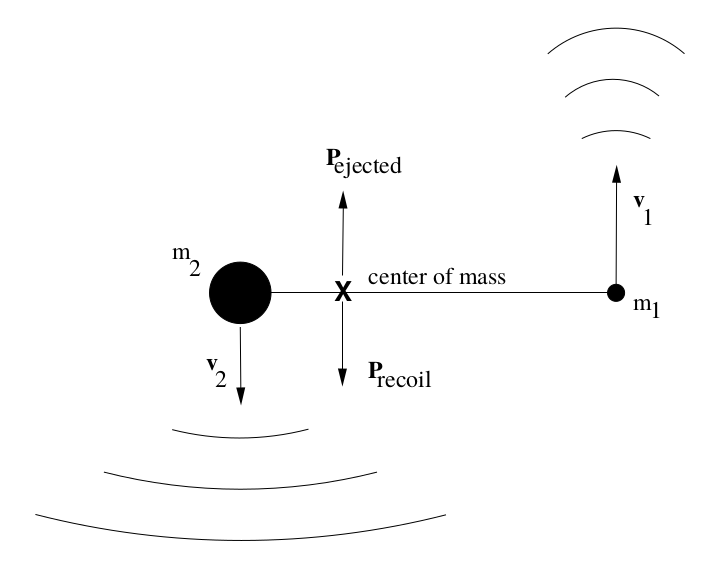
\includegraphics[width=0.6\linewidth]{Figures/binarySystem}
	\end{figure}
	
	Una forma de entender c\'omo sucede este fen\'omeno, es usando un sistema con masas desiguales. Se puede considerar dos cuerpos, uno con masa $m_1$ y otro con masa $m_2$, donde $m_2 > m_1$. En el caso cl\'asico, donde no existe ning\'un efecto nuevo, se tiene que el centro de masa orbitar\'ia alrededor de un c\'irculo. Sin embargo, cuando se tiene una onda que lleva energ\'ia y momento angular, se tiene que los cuerpos seguir\'ian una trayector\'ia en espiral, por lo cual al considerar toda una \'orbita ($\mathcal{O}$) se tendr\'ia que:
	\begin{equation}
		\int\limits_{\mathcal{O}_1} m_1\vec{v}_1dl \neq \int\limits_{\mathcal{O}_2} m_2\vec{v}_2dl 
	\end{equation}	
	
\section{Objetivo general}
%	Poner en funcionamiento el calorímetro 2277 Thermal Activity Monitor con el que se cuenta, en funcionamiento y adicionalmente calibrar el equipo para su uso en las investigaciones activas del grupo \groupname.
		
\section{Objetivos específicos}
%	\begin{itemize}
%		\item Ensamblar el equipo 2277 Thermal Activity Monitor.
%		\item Realizar el cableado y conexiones electrónicas pertinentes al mismo.
%		\item Calibración eléctrica, determinación de las señales de entrada y salida, flujo de las bombas hidráulicas y temperatura del baño.
%		\item Calibración química, determinación de la entalpía molar, energía libre de Gibbs, entropía, y constante de equilibrio, del acomplejamiento del catión bario con éter 18-corona-6.
%	\end{itemize}
%
%	\newpage

%\section{Justificación del proyecto}

%	
%	
%	
%	En general la calorimetría permite una gran variedad de análisis, muchos de ellos cuentan con aplicaciones industriales, comerciales, biológicas y químicas, permitiendo el entendimiento de las interacciones moleculares en soluciones \cite{blandamer1998titration}. Una ventaja de la calorimetría es que no es específica, ni invasiva además de no depender de las propiedades electroquímicas y ópticas de un sistema dado, siendo esto de vital importancia para las investigaciones de procesos biológicos, el estudio del crecimiento bacteriano y para la detección de compuestos biológicos \cite{winkelmann2004application}. Por otro lado la calorimetría también permite el estudio de la termodinámica en sistemas de absorción, bien sea por la universalidad de la absorción física en las superficies como catalizadores, o en procesos industriales como la separación de mezclas de gases \cite{morrison1987calorimetry}. Finalmente la calorimetría es el método clásico para la determinación de propiedades termodinámicas en las muestras, entre estas se encuentran la capacidad calorífica, la entalpía, entropía y energía libre de Gibbs, las cuales constituyen el punto de partida de gran cantidad de estudios teóricos, desarrollos y producción industrial de un compuesto químico \cite{wang2005determination, gaisford2016principles}.
%
%	El calorímetro 2277 Thermal Activity Monitor con el que cuenta el grupo de investigación se encuentra desarmado, a la espera de su ensamble y puesta en funcionamiento. Este instrumento permite monitorear una gran variedad de reacciones químicas y bioquímicas, lo anterior debido a su capacidad de cuantificar procesos exotérmicos y endotérmicos. Estas reacciones pueden ser estudiadas en el rango de 5 - 80 $^\circ$C \cite{Suurkuusk}. Este rango de temperaturas se debe al uso de un baño termostatado de 25 litros. Cuatro balones de medición independientes se encuentran sumergidos en este baño, permitiendo medidas con desviaciones de temperatura inferiores a $\pm2\times10^{-4}$ $^\circ$C, alcanzando de esta manera medidas en el rango de microvatios \cite{Suurkuusk}. Es por esta razón que poner en marcha y calibrar el equipo con el que cuenta el grupo de investigación resulta una contribución importante para el mismo, así como para el \deptname\ en general.
	
\section{Metodología}
	Las simulaciones ser\'an realizadas en el cluster de la universidad con el fin de paralelizar procesos, de forma que a haciendo uso de sus recursos se minimice el tiempo de simulación a fin de lograr la mayor cantidad de simulaciones posibles con el fin de obtener una cantidad significativa de datos de validación.
	
\section{Consideraciones éticas}
	Se manejará un repositorio de uso privado a través de Github en donde se encontrar\'an los códigos implementados en cada parte del proceso, junto con los resultados obtenidos, de forma que se asegure la reproducibilidad del modelo hallado, al mismo tiempo que se permita el seguimiento del uso de recursos. Adem\'as al mantener la informaci\'on abierta se asegura que no se están utilizando resultados obtenidos por otros investigadores de forma directa.
	
\section{Cronograma}
	\begin{table}[h]
		\centering
		\caption{Cronograma de actividades}
		\label{tb: cronograma}
		\footnotesize
		\begin{tabular}{|c|c|c|c|c|c|c|c|c|c|c|c|c|c|c|c|c|}
			\hline
			\rowcolor[HTML]{C0C0C0} 
			\cellcolor[HTML]{C0C0C0}                                       & \multicolumn{16}{c|}{\cellcolor[HTML]{C0C0C0}\textbf{Semana}} \\ \cline{2-17} 
			\rowcolor[HTML]{EFEFEF} 
			\multirow{-2}{*}{\cellcolor[HTML]{C0C0C0}\textbf{Actividades}} & \textbf{1} & \textbf{2} & \textbf{3} & \textbf{4} & \textbf{5} & \textbf{6} & \textbf{7} & \textbf{8} & \textbf{9} & \textbf{10} & \textbf{11} & \textbf{12} & \textbf{13} & \textbf{14} & \textbf{15} & \textbf{16} \\ \hline
			\cellcolor[HTML]{EFEFEF}
			\textbf{Revisión bibliográfica} & x & x & x & & & & x & x & x & x & & & & x & x & x \\ \hline
			\cellcolor[HTML]{EFEFEF}\textbf{Revisión de manuales} & x & x & x & x & & & & & & & & & & & & \\ \hline
			\cellcolor[HTML]{EFEFEF}\textbf{Ensamble del equipo} & x & x & x & x & & & & & & & & & & & & \\ \hline
			\cellcolor[HTML]{EFEFEF}\textbf{Cableado y electrónica} & & & x & x & x & x & & & & & & & & & & \\ \hline
			\cellcolor[HTML]{EFEFEF}\textbf{Calibración eléctrica} & & & & & & x & x & x & & & & & & & & \\ \hline
			\cellcolor[HTML]{EFEFEF}\textbf{Calibración química} & & & & & & & & & x & x & x & x & & & & \\ \hline
			\cellcolor[HTML]{EFEFEF}\textbf{Análisis de datos} & & & & & & & & & & & x & x & x & & & \\ \hline
			\cellcolor[HTML]{EFEFEF}\textbf{Elaboración del documento} & & & & & & & x & x & x & x & & & & x & x & x \\ \hline
			\cellcolor[HTML]{EFEFEF}\textbf{Presentación del proyecto} & & & & & & & & & & & & & & & & x \\ \hline
		\end{tabular}
	\end{table}
% !TeX spellcheck = en_US
% Chapter 1

%\chapter{Chapter Title Here} % Main chapter title
%
%\label{Chapter1} % For referencing the chapter elsewhere, use \ref{Chapter1} 

%----------------------------------------------------------------------------------------

% Define some commands to keep the formatting separated from the content 

%\newcommand{\option}[1]{\texttt{\itshape#1}}

%----------------------------------------------------------------------------------------

\chapter{Methodology}\label{ch: methodology}
	The host galaxy of the black hole is modeled as two mass distributions that are superimposed, one for dark matter and the other one for all the luminous or baryonic matter.
	\begin{figure}[h]
		\centering
		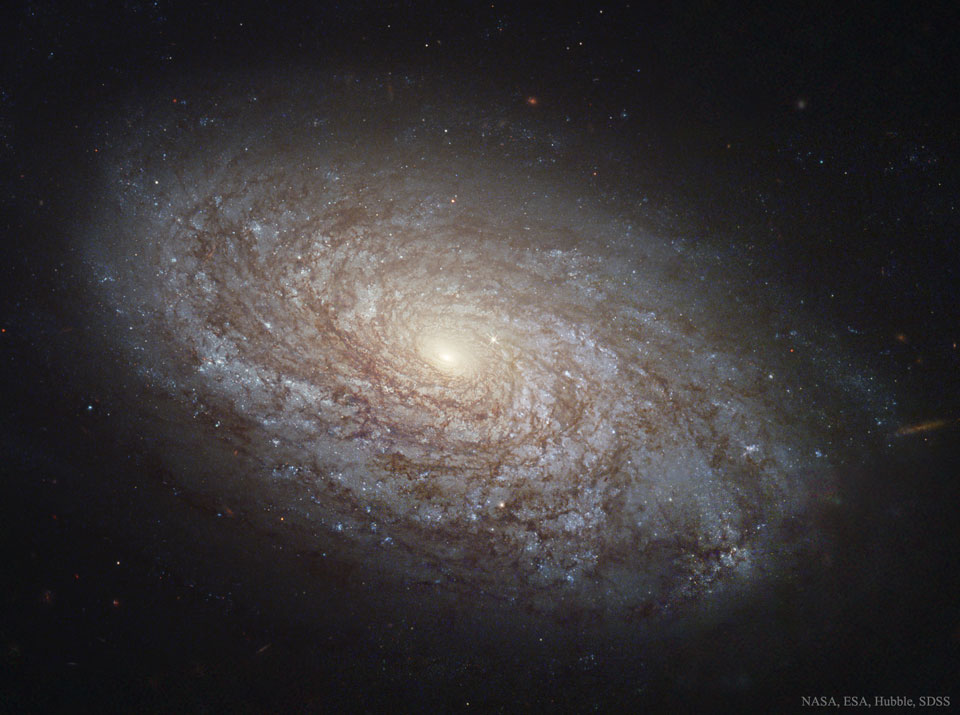
\includegraphics[width=0.8\linewidth]{Figures/NGC4414_modified}
		\caption{NGC4414 galaxy as seen by the Hubble telescope.}
	\end{figure}
	
	The dark matter halo used follows a NFW (Navarro–Frenk–White) profile, baryonic matter is divided in stars and gas, For the gas a power law profile with $r^{-2.2}$ is used, while for stars a Hernquist model is applied \cite{tanaka2009assembly, choksi2017recoiling}. The sum of all these components accounts for the total mass of the host ($M_h$), which remains constant through a simulation. The amount of baryonic matter is given by the baryonic fraction parameter ($f_b$), and the mass of stars by the stellar fraction parameter ($f_s$). Cumulative masses at the virial radius are defined as follows (Appendix A \autoref{sec: cd_vr}):
	\begin{equation}
		M_\text{DM}(R_\text{vir}) = (1 - f_b)M_h
	\end{equation}
	\begin{equation}
		M_\text{stars}(R_\text{vir}) = f_sf_bM_h
	\end{equation}
	\begin{equation}
		M_\text{gas}(R_\text{vir}) = (1 - f_s)f_bM_h
	\end{equation}
	
	Some of the simulation parameters are dependent of the cosmological model used, unless otherwise specified, all data is acquired using the $\Lambda$-CDM model with a matter density parameter $\Omega_M = 0.309$, $\Omega_\Lambda = 0.6911$, and a baryonic fraction $f_b = 0.156$ \cite{choksi2017recoiling}. Also, as \citeauthor{binney2011galactic}, argue, about 1 \% of the stellar mass of galaxies, such as The Milky Way, are contained in the stellar halo, $f_s \equiv 0.01$, unless otherwise stated.
	
	\section{Densities profiles}
		\subsection{Dark matter halo}
			For a dark matter halo following a NFW profile, the density at some distance $r$ is given by the formula:
			\begin{equation}\label{eq: dmdensity}
				\rho_\text{DM}(r) = \dfrac{\rho_0^\text{DM}}{\frac{r}{R_s}\left(1 + \frac{r}{R_s}\right)^2}
			\end{equation}
			
			Where $R_s$ and $\rho_0^\text{DM}$ are constants for a given dark matter halo. For a triaxial potential, it is said that density is constant within ellipsoids of ellipsoidal radius $m$. Using the Cartesian coordinates $x_1$, $x_2$, $x_3$ and $a_1$, $a_2$, $a_3$ the semi-axis of the ellipsoid, $m$ is defined as follows:
			\begin{equation}
				m^2(\vec{x}) \equiv a_1^2\left[\left(\dfrac{x_1}{a_1}\right)^2 + \left(\dfrac{x_2}{a_2}\right)^2 + \left(\dfrac{x_3}{a_3}\right)^2\right] = x_1^2 + \left(\dfrac{a_1}{a_2}\right)^2x_2^2 + \left(\dfrac{a_1}{a_3}\right)^2x_3^2
			\end{equation}
			
			Considering a concentration parameter $c(M_h, z)$ of dark matter in the halo, the following relation holds for the viral radius $R_\text{vir}$ and the scale radius $R_s$:
			\begin{equation}\label{eq: virialConcentration}
				R_\text{vir} = c(M_h, z)R_s
			\end{equation}
			
			Where the concentration parameter, dependence with the dark matter halo mass ($M_h$) and redshift is given by: 
			\begin{equation}
			c(M_h, z) = c_0(z)\left(\dfrac{M_h}{10^{13}M_\theta}\right)^{\alpha(z)}
			\end{equation}
			
			where $\alpha(z)$ and $c_0(z)$ were fitted using simulation data to the following functions \cite{choksi2017recoiling}:
			\begin{equation}
				c_0(z) = \dfrac{4.58}{2}\left[\left(\dfrac{1 + z}{2.24}\right)^{0.107} + \left(\dfrac{1 + z}{2.24}\right)^{-1.29}\right]
			\end{equation}
			
			\begin{equation}
				\alpha(z) = -0.0965 \exp\left(-\dfrac{z}{4.06}\right)
			\end{equation}
			
			\begin{figure}[h]
				\centering
				\includegraphics[width=0.7\linewidth]{"../Files/Week 3/darkmatter_concentration"}
				\caption{Dark matter concentration parameter as a function of the halo mass and the redshift.}
				\label{fig: dmconcentration}
			\end{figure}
			
			For a fixed halo mass, as time passes (smaller redshift), concentration of dark matter will increase, as can be shown on \autoref{fig: dmconcentration}, nevertheless for high redshifts concentration is approximately constant at $c \approx 3$ for all halos \cite{choksi2017recoiling}.
	
		\subsection{Stellar density}
			Stellar density is modeled as a Hernquist profile with half-mass radius $R_{1/2} = 0.01 R_\text{vir}$, as in \citeauthor{choksi2017recoiling}. Density for a Hernquist profile is given by \cite{hernquist1990analytical}:
			\begin{equation}\label{eq: sdensity}
				\rho_s(r) = \dfrac{f_sf_bM_h \mathcal{R}_s}{2\pi r(r + \mathcal{R}_s)^3} \qquad \text{$\mathcal{R}_s$ is known as scale length}
			\end{equation}
			
			The half-mass radius, as the name implies, is the distance at which the cumulative mass is half the total mass \cite{hernquist1990analytical}.
			\begin{equation}
				R_{1/2} = \left(1 + \sqrt{2}\right)\mathcal{R}_s = 0.01\left({\dfrac{M_hG}{100 H(t)^2}}\right)^{1/3}
			\end{equation}
			
			From which the scale length can be set as a function of the time when the kick occurs, and the mass of the host, as:
			\begin{equation}
				\mathcal{R}_s = \dfrac{0.01}{\left(1 + \sqrt{2}\right)}\left({\dfrac{M_hG}{100 H(t)^2}}\right)^{1/3} \approx 6.835\times 10^{-4}\left({\dfrac{M_h}{H(t)^2}}\right)^{1/3}
			\end{equation}
		\subsection{Gas density}
			For high redshift the baryonic profile resembles that of a gaseous galaxy, \citeauthor{choksi2017recoiling} use a constant density gas core of $r_0 = 1$ pc, followed by a power law of $r^{-n} = r^{-2.2}$. Density is described as follows: for $r \gg r_0$, $\rho_\text{gas}(r)\propto r^{-n}$ while for $r \ll r_0$, $\rho_\text{gas}(r) \approx \rho_0^\text{gas}$.
			\begin{equation}\label{eq: rdensity}
				\rho_\text{gas}(r) = \dfrac{\rho_0^\text{gas}}{\left(1 + \dfrac{r}{r_0}\right)^n}
			\end{equation}
	
	\section{Equation of motion}
		Trajectories of the kicked black holes are obtained by numerically solving the equation of motion on \autoref{eq: equationMotion}, where the first term on the right side of the equation is acceleration due to gravity, the second accounts for the drag of dynamical friction, while the third one is the deaceleration due to mass accretion of the black hole \cite{tanaka2009assembly, choksi2017recoiling}.
		\begin{equation}\label{eq: equationMotion}
			\ddot{\vec{x}}(\vec{x}, \dot{\vec{x}}) = a_\text{grav}(\vec{x})\hat{x} + \left(a_\text{DF}(\vec{x}, \dot{\vec{x}})-\dot{x}\dfrac{\dot{M_\bullet}(x, \dot{x})}{M_\bullet}\right)\dot{\hat{x}} \qquad \text{where $M_\bullet$ is the black hole mass}
		\end{equation}
		
		\subsection{Dynamical friction}
			As the black hole travels through the galaxy, dark matter, stars and gaseous materials from the medium interact with the black hole adding a drag force due to friction. Drag force is different in nature depending on its source, collisionless components, such as dark matter and stars, apply a drag force to the black hole that follows the standard Chandrasekhar formula \cite{binney2011galactic, madau2004effect, tanaka2009assembly, choksi2017recoiling}.
			\begin{equation}\label{eq: df_cl}
				a_\text{DF}^\text{cl}(\vec{x}, \dot{\vec{x}}) = -\dfrac{4\pi G^2}{\dot{x}^2} M_\bullet\rho(\vec{x})\ln\Lambda\left(\erf{X} - \dfrac{2}{\sqrt{\pi}}Xe^{-X^2}\right)\text{, } \quad \rho(\vec{x}) = \rho_\text{DM}(\vec{x}) + \rho_\text{stars}(\vec{x})
			\end{equation}
			\begin{equation}
				X \equiv \dfrac{|\dot{x}|}{\sqrt{2}\sigma_\text{DM}} \qquad \text{with } \sigma_\text{DM} = \sqrt{\dfrac{GM_\text{DM}}{2R_\text{vir}}}
			\end{equation}
			
			$\sigma_\text{DM}$ is called the local velocity dispersion of the dark matter halo, and since varies little over the entire host, can be taken as constant \cite{tanaka2009assembly, choksi2017recoiling}. The Coulomb logarithm ($\ln\Lambda$) is not known but authors take it in the range of 2 - 4 \cite{choksi2017recoiling}. Gas on the other hand is collisional, special care must be taken since gas can cool behind a passing object, such as a black hole \cite{choksi2017recoiling}. A hybrid model for the drag force was proposed by \citeauthor{tanaka2009assembly}, in which both subsonic and supersonic velocities are possible. To do so, a mach number was defined as:
			\begin{equation}
				\mathcal{M}(\dot{x}) \equiv \dfrac{|\dot{x}|}{c_s}
			\end{equation}
			
			where $c_s$ is the local sound speed, which depends on local temperature. It was found that temperature inside the halo varies less than a factor of 3, thus on the simulation it is assumed that the entire halo is isothermal at the virial temperature ($T_\text{vir}$) \cite{choksi2017recoiling}. The isothermal sound speed is \cite{barkana2001beginning}:
			\begin{equation}\label{eq: soundSpeed}
				c_s = \sqrt{\dfrac{\gamma R}{\mathcal{M}_w}T_\text{vir}} = \sqrt{\dfrac{\gamma R}{\mathcal{M}_w}\left(\dfrac{\mu m_p G M_h}{2k_BR_\text{vir}}\right)} = \sqrt{\dfrac{\gamma R\mu m_pG}{2\mathcal{M}_wk_B}} \sqrt{\dfrac{M_h}{R_\text{vir}}} \approx 0.614 \sqrt{\dfrac{M_h}{R_\text{vir}}}\text{ kpcGyr$^{-1}$}
			\end{equation}
			
			where $\mu$ is the value of the mean molecular weight of the gas ($\mathcal{M}_w$), $m_p$ is the proton mass and $\gamma$ is the adiabatic index \cite{barkana2001beginning}. Approximating the gas to a monoatomic one $\gamma \approx 5/3$, yields the last expression on \autoref{eq: soundSpeed}. By knowing $\mathcal{M}$, the acceleration caused by gas can be written as \cite{tanaka2009assembly, choksi2017recoiling}:
			\begin{equation}\label{eq: df_c}
				a^\text{c}_\text{DF}(\vec{x}, \dot{\vec{x}}) = -\dfrac{4\pi G^2}{\dot{x}^2}M_\bullet\rho_\text{gas}(\vec{x})f(\mathcal{M})
			\end{equation}
			
			with
			\begin{equation}
				f(\mathcal{M}) = \left\{
				\begin{matrix}
				0.5\ln\Lambda \left[\erf{\dfrac{\mathcal{M}}{\sqrt{2}}} - \sqrt{\dfrac{2}{\pi}}\mathcal{M}e^{-\mathcal{M}^2/2}\right]& \text{if $\mathcal{M} \leq 0.8$}\\
				1.5\ln\Lambda \left[\erf{\dfrac{\mathcal{M}}{\sqrt{2}}} - \sqrt{\dfrac{2}{\pi}}\mathcal{M}e^{-\mathcal{M}^2/2}\right] & \text{if $0.8 < \mathcal{M} \leq \mathcal{M}_{eq}$}\\
				0.5\ln\left(1 - \mathcal{M}^{-2}\right) + \ln\Lambda & \text{if $\mathcal{M} > \mathcal{M}_{eq}$}
				\end{matrix}
				\right.
			\end{equation}
			
			$M_{eq}$ is the mach number that fulfills the following equation:
			\begin{equation}\label{eq: machEq}
				\ln\Lambda\left[1.5\left(\erf{\dfrac{\mathcal{M}}{\sqrt{2}}} - \sqrt{\dfrac{2}{\pi}}\mathcal{M}e^{-\mathcal{M}^2/2}\right) - 1\right] - 0.5\ln\left(1 - \mathcal{M}^{-2}\right) = 0
			\end{equation}
			
			Numerically solving \autoref{eq: machEq}, yields $M_{eq} \approx 1.731$ for a value of the Coulomb logarithm $\ln\Lambda = 2.3$. The full acceleration due to dynamical friction is given by the sum of the noncollisional drag on \autoref{eq: df_cl} and \autoref{eq: df_c}:
			\begin{equation}
				a_\text{DF}(\vec{x}, \dot{\vec{x}}) = a_\text{DF}^\text{cl}(\vec{x}, \dot{\vec{x}}) + a_\text{DF}^\text{c}(\vec{x}, \dot{\vec{x}})
			\end{equation}
		
		\subsection{Accretion onto the black hole}
			As the black hole accretes matter from the surroundings, an acceleration appears, due to the second law of Newton:
			\begin{equation}
				\vec{F} = \dfrac{d\vec{P}}{dt} = \dot{\vec{x}}\dot{M}_\bullet + M_\bullet\ddot{\vec{x}}
			\end{equation}
			
			By considering conservation of momentum:
			\begin{equation}
				\ddot{\vec{x}} = - \dot{\vec{x}}\dfrac{\dot{M}_\bullet}{M_\bullet}
			\end{equation}
			
			Two schemes describe the speed at which the black hole gains mass, on the first one the black hole undergoes Bondi-Hoyle-Littleton accretion \cite{tanaka2009assembly, choksi2017recoiling}:
			\begin{equation}
				\dot{M}_\bullet^\text{BHL}(\vec{x}, \dot{\vec{x}}) = \dfrac{4\pi G^2 \rho_G(\vec{x})M^2_\bullet}{\left(c_s^2 + \dot{x}^2\right)^{3/2}} \qquad \text{with } \rho_B(\vec{x}) = \rho_\text{stars}(\vec{x}) + \rho_\text{gas}(\vec{x})
			\end{equation}
			
			There is a limit of accretion for the black hole given by the Eddington luminosity:
			\begin{equation}\label{eq: eddington}
				\dot{M}_\bullet^\text{Edd} = \dfrac{(1 - \epsilon)M_\bullet}{\epsilon t_\text{Edd}} \qquad \epsilon = 0.1, \quad t_\text{Edd} = 0.44 \text{ Gyr}
			\end{equation}
			
			Final accretion rate is given by:
			\begin{equation}
				\dot{M}_\bullet(\vec{x}, \dot{\vec{x}}) = \left\{
				\begin{array}{lc}
				\dot{M}_\bullet^\text{BHL}(\vec{x}, \dot{\vec{x}}) & \text{if $\dot{M}_\bullet^\text{BHL} < \dot{M}_\bullet^\text{Edd}$} \\
				\dot{M}_\bullet^\text{Edd} & \text{else}
				\end{array}
				\right.
			\end{equation}
	
	\subsection{Initial conditions and numerical integration}
		For all simulations the virial radius remains constant through the simulation. The virial radius is fixed at the start of every simulation depending on the redshift at which the kick occurs, the chosen densities profiles and the mass of the host galaxy. Sound speed also remains constant for a simulation, as it depends on $R_\text{vir}$ and the mass of the host. Cosmological acceleration is ignored at all times as in \citeauthor{tanaka2009assembly}, as it has been found that it only marginally affects black hole orbits \cite{choksi2017recoiling}. The initial position of the black hole is always $\vec{x} = (0, 0, 0)$ kpc.
		
		Numerical integration is carried out using a leapfrog scheme on REBOUND with the C programming language \cite{larson2017modeling}, with time steps of a thousand years, the simulations are stopped when the system destabilizes and starts gaining energy, due to singularities at $x \rightarrow 0$ and $\dot{x} \rightarrow 0$, or if they simply last more than the age of the universe. 
		
	\section{Definitions}
		\subsection{Escape velocity}
			Minimum initial velocity required for the maximum distance of a single orbit of the black hole to stay outside $0.01R_\text{vir}$ by $z = 0$, $z = 6$ or 10 \% of the age of the universe at the moment of the kick \cite{tanaka2009assembly, choksi2017recoiling}.
		
		\subsection{Time of return}
			Time required by the black hole to orbit with maximum distances of less than  $0.01R_\text{vir}$.
			
	\section{Spherical setup}
	\subsection{Virial radius}
		Since all of the density profiles are spherically symmetrical, it follows from \autoref{eq: R_vir_def} that:  
		\begin{equation}
		\dfrac{M_h}{4/3\pi R_\text{vir}^3} = 75\dfrac{H(t)^2}{\pi G}
		\end{equation}
		\begin{equation}
		R_\text{vir} = \left({\dfrac{M_hG}{100 H(t)^2}}\right)^{1/3}
		\end{equation}
	
	\subsection{Dark matter halo}
		For a dark matter halo following a NFW profile, the cumulative mass $M_\text{DM}(r)$ within some radius $r$ is given by the integral of the density over a volume. Since \autoref{eq: dmdensity} is spherically symmetrical, the only dependance of the integral is with distance. On \autoref{eq: cumulativeDM} the $r'^2$ comes from the Jacobian of spherical coordinates, and the $4\pi$ from the solid angle.
		\begin{equation}\label{eq: cumulativeDM}
			M_{DM}(r) = \int\limits_0^{r} 4\pi {r'}^2\rho_\text{DM}(r')dr' = 4\pi\rho_0^\text{DM}R_s^3\left[\ln\left(\dfrac{R_s + r}{R_s}\right) - \dfrac{r}{R_s + r}\right]
		\end{equation}
		
		By using \autoref{eq: virialConcentration} one can obtain the value of $\rho_0^\text{DM}$ by evaluating \autoref{eq: cumulativeDM} at $R_\text{vir}$.
		\begin{equation}\label{eq: dmM_virial}
		M_\text{DM}(R_\text{vir}) = 4\pi\rho_0^\text{DM}R_s^3 \left[\ln\left(\dfrac{R_s + c(M_h, z)R_s}{R_s}\right) - \dfrac{c(M_h, z)R_s}{R_s + c(M_h, z)R_s}\right] = (1 - f_b)M_h
		\end{equation}
		\begin{equation}\label{eq: rho0dm}
		\rho_0^\text{DM} = \dfrac{(1 - f_b)M_h}{4\pi \left(\dfrac{R_\text{vir}}{c(M_h, z)}\right)^3 \left[\ln\left(1 + c(M_h, z)\right) - \dfrac{c(M_h, z)}{1 + c(M_h, z)}\right]}
		\end{equation}
	
	\subsection{Stellar profile}		
		Integrating \autoref{eq: sdensity} from $0$ to $r$ yields:
		\begin{equation}
			M_s(r) = \dfrac{f_sf_bM_h r^2}{(r + \mathcal{R}_s)^2}
		\end{equation}
	
	\subsection{Gas profile}		
		The cumulative mass is found by integrating \autoref{eq: rdensity} in spherical coordinates.
		\begin{equation}
			\begin{array}{rl}
			M_\text{gas}(r) 
			& = 4\pi\rho_0^\text{gas} r_0^3\int\limits_{0}^{u}\dfrac{u'^2}{(1 + u')^n}du' \\
			& = 4\pi\rho_0^\text{gas} r_0^3\left(u + 1\right)^{-n}\dfrac{-(u + 1)(nu)^2 + 2[(u + 1)^n - u^3-1] + nu[3u^2 + u - 2]}{(n - 3)(n - 2)(n - 1)}
			\\
			& \text{where $u = r/r_0$, for $u \leq 0$ and $n \neq {1, 2, 3}$}
			\end{array}
		\end{equation}
		
		The value of the constant $\rho_0^\text{gas}$ is found using a similar process as in \autoref{eq: dmM_virial} and \ref{eq: rho0dm}.
		\begin{equation}
			\rho_0^\text{gas} = \dfrac{(1 - f_s) f_bM_h}{(M_\text{gas}(R_\text{vir}) / \rho_0^\text{gas})}
		\end{equation}
		
		All of the profiles are shown on \autoref{fig: massprofiles}, where the effect of the stellar fraction can be seen.
		
		\begin{figure}[h]
			\centering
			\begin{subfigure}[b]{0.49\textwidth}
				\includegraphics[width=\textwidth]{"../Files/Week 6/density_mass_fs01"}
				\caption{Stellar fraction $f_s = 0.01$.}
				\label{fig: baryonicprofilehigh}
			\end{subfigure}
			~ 
			\begin{subfigure}[b]{0.49\textwidth}
				\includegraphics[width=\textwidth]{"../Files/Week 6/density_mass_fs3"}
				\caption{Stellar fraction $f_s = 0.30$.}
				\label{fig: baryonicprofilelow}
			\end{subfigure}
			\caption{Mass distributions for $R_\text{vir} = 0.69$ kpc (red line), $c = 4$, and $f_b = 0.156$.}
			\label{fig: massprofiles}
		\end{figure}
	
	\section{Triaxial setup}
		\begin{figure}[h]
			\centering
			\begin{subfigure}[t]{0.49\textwidth}
				\includegraphics[width = \textwidth]{"../Files/Week 7/symmetric"}
				\caption{Spherical case}
				\label{fig: symmetricDensity3d}
			\end{subfigure}
			~ 
			\begin{subfigure}[t]{0.49\textwidth}
				\includegraphics[width=\textwidth]{"../Files/Week 7/triaxial"}
				\caption{Triaxial case with ($a_1$:$a_2$:$a_3$) = (1:0.5:0.3)}
				\label{fig: triaxialDensity3d}
			\end{subfigure}
			\begin{subfigure}[t]{0.6\textwidth}
				\includegraphics[width=\textwidth]{"../Files/Week 7/ellipsoid_"}
				\caption{Equicentred ellipsoids with ($a_1$:$a_2$:$a_3$) = (1:0.5:0.3)}
			\end{subfigure}
			\caption{Dark matter densities comparison between spherical and triaxial cases.}
			\label{fig: symmetricTriaxial}
		\end{figure}
	
		The host galaxy is modeled as a dark matter halo, stars and gas, just as the spherical case. Much of the profiles for each of the components remains the same, the only difference is that a thin shell of uniform density will have the geometry of an ellipsoid, and not that of a sphere. This is achieved by defining an ellipsoid radius $m$, that can be replaced for the spherical radius $r$, on equations \ref{eq: dmdensity}, \ref{eq: sdensity} and \autoref{eq: rdensity}, as can be seen on \autoref{fig: symmetricTriaxial}. 
		
		A thin shell, whose inner and outer skins are the surfaces $m$ and $m + \delta m$ is described by \autoref{eq: m2}, where $\tau \geq 0$ labels the surfaces \cite{binney2011galactic}.
		\begin{equation}\label{eq: m2}
		m^2(\vec{x}, \tau) = a_1^2\left(\frac{x_1^{2}}{\tau + a_{1}^{2}} + \frac{x_2^{2}}{\tau + a_{2}^{2}} + \frac{x_3^{2}}{\tau + a_{3}^{2}}\right)
		\end{equation}
		
		Densities are used for the calculation of the dynamical friction and accretion onto the black hole. Although one might think that by integrating the density over an elliptical volume, the acceleration due to gravity would be given by $a_\text{grav} = GM(m)/m^2$, the later is not true because two points $(x_1, x_2, x_3)$ and $(x_1', x_2', x_3')$ might have the same cumulative mass at $m$ (black line), but the effective gravitational mass acting at each point is completely different (blue and orange lines) as it is shown in \autoref{fig: triaxial_mass_issue}.
		\begin{figure}[h]
			\centering
			\includegraphics[width = 0.4\linewidth]{"../Files/Week 7/triaxial_mass_issue"}
			\caption{Although the cumulative mass at the orange and blue dots is the same, the effective gravitational mass is different.}
			\label{fig: triaxial_mass_issue}
		\end{figure}
	
		Because of this, the potential due to a given triaxial density must be found. Calculating the gravitational potential for such configuration, challenged some great minds of the XVIII and XIX centuries \cite{binney2011galactic}. To do so, the contributions of all ellipsoidal shells that make up the profile are taken into account, following \citeauthor{binney2011galactic}:
		\begin{equation}
			\psi(m) \equiv \int\limits_{0}^{m^2} \rho(m'^2)dm'^2 = \int\limits_{0}^{m} 2m'\rho(m')dm' 
		\end{equation}
		
		The potential of any body in which $\rho = \rho(m^2)$ is \cite{binney2011galactic}:
		\begin{equation}\label{eq: generalPotential}
		\Phi(\vec{x}) = -\pi G \dfrac{a_2a_3}{a_1}\int\limits_{0}^{\infty}\dfrac{\psi(\infty) - \psi(m)}{\sqrt{(\tau + a_1^2)(\tau + a_2^2)(\tau + a_3^2)}}d\tau \qquad m = m(\vec{x}, \tau)
		\end{equation}
		\begin{table}[h]
			\centering
			\caption{$\psi$ values for the studied density profiles}
			\begin{tabular}{c|c}
				\hline
				\textbf{Profile} & $\psi(\infty) - \psi(m)$ \\
				\hline
				\rule{0pt}{4ex} 
				\textbf{NFW} & $\dfrac{2R_s^3\rho_0^\text{DM}}{R_s + m(\vec{x}, \tau)}$\\
				%				\hline
				\textbf{Hernquist} & $\dfrac{M_s\mathcal{R}_s}{2\pi\left(\mathcal{R}_s + m(\vec{x}, \tau)\right)^2}$ \\
				%				\hline
				\textbf{Power-law} & $\dfrac{2 \rho_0^\text{gas} \left(\frac{m(\vec{x}, \tau) + r_{0}}{r_{0}}\right)^{- n} \left(m(\vec{x}, \tau) + r_{0}\right) \left(m(\vec{x}, \tau) \left(n - 1\right) + r_{0}\right)}{\left(n - 2\right) \left(n - 1\right)}$
				\\
				\hline
			\end{tabular}
		\end{table}
		
		Most of the triaxials potentials cannot be analytically integrated, nevertheless it can be done numerically. Since the gravitational acceleration is given by the gradient of the potential, to numerically calculate the gradient, a total of 6 numerical integrals must be done (two for each dimension, and then numerically differentiate). Another option is to take advantage of the fact that $\vec{x}$ and $\tau$ are independent variables, thus:
		\begin{equation}
			\nabla \int f(\vec{x}, \tau)d\tau = \int [\nabla f(\vec{x}, \tau)] d\tau
		\end{equation}
		
		By doing this, the number of numerical integrals reduces to 3. Defining a vector $\vec{\phi}$, whose components are given by:
		\begin{equation}
			\phi_i(x_i, \tau) = \dfrac{x_i}{\left(\tau + a_i^2\right)^{\frac{3}{2}} \prod\limits_{i \neq j}^3\sqrt{\tau + a_j^2}}, \qquad \vec{\phi}(\vec{x}, \tau) = (\phi_1(x_1, \tau), \phi_2(x_2, \tau), \phi_3(x_3, \tau))
		\end{equation}
		
		Potentials for each of the components of the galaxy are found by finding $\psi(\infty) - \psi(m)$ and replacing on \autoref{eq: generalPotential}.
		
		
	
		\begin{table}[h]
			\centering
			\caption{$\nabla\Phi(\vec{x})$ values for the studied density profiles}
			\label{tb: gradients}
			\begin{tabular}{c|c}
				\hline
				\textbf{Profile} & $\nabla \Phi(\vec{x})$\\
				\hline
				\rule{0pt}{4ex}
				\textbf{NFW} & $2 \pi G R_{s}^{3}\rho_0 a_{1} a_{2} a_{3} \displaystyle\int\limits_{0}^{\infty}
				\dfrac{\vec{\phi}(\vec{x}, \tau) d\tau}{m(\vec{x}, \tau)\left(R_{s} + m(\vec{x}, \tau)\right)^{2}}$ \\
				%				\hline
				\textbf{Hernquist} &  $G M_{s} \mathcal{R}_s a_{1} a_{2} a_{3} \displaystyle\int\limits_{0}^{\infty} \frac{ \vec{\phi}(\vec{x}, \tau) d\tau}{m(\vec{x}, \tau)\left(\mathcal{R}_s + m(\vec{x}, \tau)\right)^{3}}$ \\
				%				\hline
				\textbf{Power-law} & $2 \pi G a_{1} a_{2} a_{3}  \rho_{0}^\text{gas}  \displaystyle\int\limits_{0}^{\infty}\vec{\phi}(\vec{x}, \tau)\left(\dfrac{r_{0}}{m(\vec{x}, \tau) + r_{0}}\right)^{n}d\tau$\\
				\hline
			\end{tabular}
			
		\end{table}	
		
		Two Gaussian quadrature integration schemes are tested, Gauss-Legendre and Gauss-Laguerre. Both schemes rely on the use of orthogonal polynomials whose roots yield the nodes $x_i$ at which a function is evaluated, multiplied by a weighting value $w_i$ in order to calculate its integral as in \autoref{eq: gauss}, where $k$ is the degree of the polynomial used.
		\begin{equation}\label{eq: gauss}
			\int\limits_{a}^{b} w(x)f(x)dx \approx \sum_{i = 1}^{k}w_i f(x_i), \qquad \text{where $w(x)$ is a weighting function}
		\end{equation}
		
		\begin{table}[h]
			\centering
			\caption{Weighing functions and intervals of integration for Gauss quadratures}
			\begin{tabular}{ccc}
				\hline
				\textbf{Interval} & \textbf{Weighting function} & \textbf{Orthogonal polynomials} \\
				\hline
				$[-1, 1]$ & $1$ & Legendre \\
				$[0, \infty)$ & $e^{-x}$ & Laguerre \\
				\hline
			\end{tabular}
		\end{table}
		
		To make the integral proper, for the Gauss-Legendre quadrature, the following change of variable is done:
		\begin{equation}\label{eq: changeVariable}
			\omega = \dfrac{\tau^\gamma}{\tau^\gamma + 1}, \qquad \tau = \left(\frac{\omega}{1-\omega}\right)^{\frac{1}{\gamma}}, \qquad d\tau = \dfrac{\left(- \frac{\omega}{\omega - 1}\right)^{\frac{1}{\gamma}}}{\gamma \omega \left(- \omega + 1\right)} d\omega, \qquad \gamma > 0
		\end{equation} 
		
		By using \autoref{eq: changeVariable}, the new interval is $[0, 1]$, thus, to use the Gauss-Legendre, the following change is done:
		\begin{equation}
			\int\limits_{0}^{1}f(x)dx = \dfrac{1}{2}\int\limits_{-1}^{1}f\left(\dfrac{x + 1}{2}\right)dx \approx \dfrac{1}{2}\sum_{i = 1}^{k}w_if\left(\dfrac{x + 1}{2}\right)
		\end{equation}
		
		In the case of Gauss-Laguerre a weighting function is required, since non of the integrals on \autoref{tb: gradients} has a term of the form $e^{-\tau}$, it is introduced by multiplying and dividing all expressions by $e^{\tau}$.
		\begin{equation}
			\int\limits_{0}^{\infty}e^{-x}e^{x}f(x) = \int\limits_{0}^{\infty}e^{-x}g(x) = \sum_{i = 1}^{k}w_i g(x), \qquad \text{where g$(x) = e^xf(x)$}
		\end{equation}
		
		To test the exactitude of the numerical approximation, integrals on \autoref{tb: gradients} are compared with the potential generated by the spherical analog in which $\nabla\Phi = GM(r)/r^2$ by making all semi-axis equal to 1.
		
		\begin{figure}[h]
			\centering
			\begin{subfigure}[t]{0.45\textwidth}
				\includegraphics[width = \textwidth]{"../Files/Week 8/gamma_error"}
				\caption{Error associated with the value of $\gamma$.}
				\label{fig: gammaError}
			\end{subfigure}
			~ 
			\begin{subfigure}[t]{0.45\textwidth}
				\includegraphics[width=\textwidth]{"../Files/Week 8/scheme_error"}
				\caption{Comparison of the error due to Gauss-Legendre (segmented lines, $\gamma = 0.2$) and Gauss-Laguerre integration schemes.}
				\label{fig: Gscheme_error}
			\end{subfigure}
			\caption{Error assessment of the numerical integrators, at $\vec{x} = (1, 0, 0)$ kpc.}
		\end{figure}
	
		Since $\gamma$ is a free parameter in the Gauss-Legendre scheme, it must be optimized, results on \autoref{fig: gammaError} show a stability region for all potentials close to $\gamma = 0.2$. On \autoref{fig: Gscheme_error}, a comparison of the error for both Gauss schemes is made, finding that Gauss-Legendre is better for all potentials when the degree of the polynomial used is bigger than 10, and that after $k \approx 50$ there is no variation on the error with Gauss-Legendre.
		\begin{figure}[!h]
			\centering
			\begin{subfigure}[t]{0.4\textwidth}
				\includegraphics[width = \textwidth]{"../Files/Week 8/error"}
				\caption{Errors on potential}
				\label{fig: potentialErrors}
			\end{subfigure}
			~ 
			\begin{subfigure}[t]{0.4\textwidth}
				\includegraphics[width = \textwidth]{"../Files/Week 7/symmetric_triaxial"}
				\caption{Cumulative errors on simulations}
				\label{fig: simulationErrors}
			\end{subfigure}
			\caption{Differences for analytical and numerical integration of the potentials gradients.}
			\label{fig: numericalErrors}
		\end{figure}
	
		Furthermore, error is not constant with distance, as can be seen on \autoref{fig: potentialErrors}. In particular, the numerical error in the calculation of the gradient of the potential is associated to the gas, causing the orbits to change slightly due to cumulative errors in each time step.
% !TeX encoding = UTF-8
% !TeX spellcheck = en_US
% Chapter 1

%\chapter{Chapter Title Here} % Main chapter title
%
%\label{Chapter1} % For referencing the chapter elsewhere, use \ref{Chapter1} 

%----------------------------------------------------------------------------------------

% Define some commands to keep the formatting separated from the content
%\newcommand{\option}[1]{\texttt{\itshape#1}}

%----------------------------------------------------------------------------------------
\chapter{Results and discussion}
	\section{Spherical study}
	For a single simulation, the following data are saved: iteration time, current position, speed, and the black hole mass. With this information, accelerations and densities can be later reconstructed as on \autoref{fig: overallOutput}.
	\begin{figure}[h]
		\centering
		\includegraphics[width = 0.52\textwidth]{"../Files/Week 6/properties_s02v70"}
		\caption{Upper two plots show the output of a single simulation, while the lower one shows most the local properties per data point.}
		\label{fig: overallOutput}
	\end{figure}
	
	\subsection{Effect of the baryonic fraction}
	The cosmological model used has two main effects in the simulations. The virial radius depends on the value of the Hubble parameter, that changes for different red-shifts and cosmological models (\autoref{fig: hubbleTime}), and the amount of matter in the universe. This effect can be seen on \autoref{fig: baryonicfraction}, where results for a galaxy made by dark matter only allow the black hole to get further away, and dissipate energy slower.
	\begin{figure}[h]
		\centering
		\includegraphics[width = 0.7\textwidth]{"../Files/Week 5/baryonic_fraction_comparison"}
		\caption{Effect of the baryonic fraction in the orbit of the black hole.}
		\label{fig: baryonicfraction}
	\end{figure}

	Three factors need to be taken into account to explain these results. First, dynamical friction due to collisional matter has an important impact on the trajectories followed by the black hole, as can be seen with the green line of \autoref{fig: overallOutput} ($a_\text{DF}$). Second, as there is no baryonic mass to accrete, the black hole does not decrease its speed because of momentum conservation, thus there is no contribution to the black hole's acceleration of the third term in \autoref{eq: equationMotion}. Lastly, as seen in \autoref{fig: massprofiles} at short distances, the cumulative mass of the galaxy is governed by stars, from which it is expected for the black hole to reach further regions of space if there are no stars, because of the smaller potential.
		
	\subsection{Effect of the power law exponent}	
		Many studied galaxies have luminosity profiles that follow a power law in distance. Nevertheless, power law density profiles have the exponent $n$ as free parameter, although it is expected to be approximate to 2, as rotation curves of galaxies at large radii show that the rotation speed of stars becomes independent of their distance to the center \cite{binney2011galactic}. This can be shown by considering a system in which density drops with radius as a function of a $n$ power:
		\begin{equation}
			\rho(r) = \rho_0^\text{gas}\left(\dfrac{r_0}{r}\right)^n
		\end{equation}
		
		The cumulative mass at a radius $r$ from the center of such distribution is:
		\begin{equation}\label{eq: centripetalMass}
			M(r) = 4\pi\rho_0^\text{gas}r_0^n\int\limits_{0}^r \mathcal{R}^2\mathcal{R}^{-2}d\mathcal{R} = \dfrac{4\pi\rho_0^\text{gas}r_0^n}{3-n}r^{3-n}
		\end{equation}
		
		Furthermore, by considering the centripetal acceleration caused by gravity:
		\begin{equation}\label{eq: centripetalForce}
			F = \dfrac{mM(r)G}{r^2} = \dfrac{4\pi m\rho_0^\text{gas}r_0^nG}{3-n}r^{1-n} = ma = \dfrac{mv^2(r)}{r}
		\end{equation}
		The speed at a distance $r$ is then:
		
		\begin{equation}\label{eq: centripetalSpeed}
			v(r) = \sqrt{\dfrac{4\pi \rho_0^\text{gas}r_0^nG}{3-n}r^{2-n}}
		\end{equation}
		
		\autoref{eq: centripetalSpeed} shows that if $n = 2$, $v(r) = v$, which means that the rotation speed becomes independent of $r$. Nevertheless, as \autoref{eq: centripetalMass} and \autoref{eq: centripetalForce} reveal, the value of $n$ strictly depends on the force generated by gravity, which in turn depends on the mass distribution within the galaxy. By taking the gradient of the potentials on \autoref{tb: potentials}, one can see that the NFW and Herquist profiles generate forces almost but not equally proportional to $r^{-2}$.
		
		Moreover, many galaxies show a smooth transition between two distinct power laws, one for small radii, and another one for large distances \cite{binney2011galactic}. The general form for densities following a double power law is:
		\begin{equation}
			\rho(r) = \dfrac{\rho_0}{\left(\dfrac{r}{a}\right) ^ \alpha \left(1 + \dfrac{r}{a}\right) ^ {\beta - \alpha}}
		\end{equation}
		
		From which one obtains all of the densities profiles used, as NFW is a double power law with $(\alpha, \beta) = (1, 3)$, Hernquist $(1, 4)$ and for gases, $(0, n)$, as seen in equations \ref{eq: dmdensity}, \ref{eq: sdensity} and \ref{eq: rdensity}. Double power laws have an advantage over piecewise-defined functions, as they are smooth for all distances. 		
		\begin{figure}[h]
			\centering
			\begin{subfigure}[t]{0.49\textwidth}
				\includegraphics[width = \textwidth]{"../Files/Week 6/power_law"}
				\caption{Effect of the power law exponent on the orbits of the black hole.}
				\label{fig: powerLawOrbits}
			\end{subfigure}
			~ 
			\begin{subfigure}[t]{0.49\textwidth}
				\includegraphics[width=\textwidth]{"../Files/Week 6/power_law_density"}
				\caption{Density and mass of the host galaxy as a function of the distance from the center, for different exponents.}
				\label{fig: powerLawDensities}
			\end{subfigure}
			\caption{Properties of the power law exponent.}
			\label{fig: powerLaw}
		\end{figure}
	
		Since $n$ is not fixed, simulations were made for a range of exponents in the power law. Results can be seen in \autoref{fig: powerLaw}, were a clear influence of the exponent can be seen. A confirmation that everything went the way it is supposed to, is that cumulative masses for all of the exponents have the same value at the virial radius (red line in \autoref{fig: powerLawDensities}). At this same distance, the behavior of the mass for each exponent changes, as smaller values of $n$ have a bigger cumulative masses from there on. At any other point, the density for bigger values of $n$ is greater, which means that both dynamical friction and accretion rates increase for the black hole as $n$ get bigger. Also, as $n$ becomes greater, cumulative masses increase, yielding a higher gravitational potential. Both of these effects, take part in the observed results in \autoref{fig: powerLawOrbits}, in which, higher values of $n$ increase return times.
		
		There are some spiral galaxies from which an exponent of 2.6 has been calculated as in NGC 253 \cite{sorai2000distribution}. Others authors have made simulations for black hole escape velocities with $n = 2.2$ \cite{tanaka2009assembly, choksi2017recoiling}. It is from these references, from which the value of $n = 2.2$ for most simulations was selected.
		
	\subsection{Effect of the stellar fraction}
		As was mentioned before, the mass of a galaxy at low distances from its center, is ruled by the amount of stars. Because of this, a study of the dependence of the return times with stellar fraction, and initial speed was carried on. For that, simulations with initial speeds from 55 to 90 kpc/Gyr were lunched, for stellar fractions ranging from 1 \% to 10 \%. In order to normalize speeds, initial speeds are divided by the escape velocity. By considering the potential energy at the edge of the galaxy, and the initial energy of the black hole, the escape velocity is written as:
		\begin{equation}
			v_\text{escape} = \sqrt{2 \left(\Phi(R_\text{vir}) - \Phi(r_0)\right)}
		\end{equation}
		
		Results from the simulations can be seen on \autoref{fig: stellarfraction}, where a linear behavior below the escape speed is common for all stellar fractions. As the initial velocities approximate 1.3, an exponential growth is seen, and return times become divergent.
		\begin{figure}[h]
			\centering
			\includegraphics[width = 0.7\textwidth]{"../Files/Week 10/returntimes_speed"}
			\caption{Return times of the black hole for different initial speeds and stellar fractions.}
			\label{fig: stellarfraction}
		\end{figure}
	
		Return times are thus fitted to the following equation:
		\begin{equation}\label{eq: fitTr}
			\log_{10}(T_\text{return}) = [a(f_s) v + b(f_s)] + \dfrac{c(f_s)}{v - 1.3}
		\end{equation}
		
		Where the first term accounts for the linear behavior and the last for the divergence at high velocities. Using the information in \autoref{fig: stellarfraction}, coefficients in \autoref{eq: fitTr} are calculated for each stellar fraction. Later, with the value of the coefficients, a second fit is made for $a(f_s), b(f_s), c(f_s)$.
		
		\begin{figure}[h]
			\centering
			\begin{subfigure}[t]{0.4\textwidth}
				\includegraphics[width = \textwidth]{"../Files/Week 10/a"}
				\caption{}
%				\label{fig: symmetricDensity3d}
			\end{subfigure}
			~ 
			\begin{subfigure}[t]{0.4\textwidth}
				\includegraphics[width=\textwidth]{"../Files/Week 10/b"}
				\caption{}
%				\label{fig: triaxialDensity3d}
			\end{subfigure}
			\begin{subfigure}[t]{0.4\textwidth}
				\includegraphics[width=\textwidth]{"../Files/Week 10/c"}
				\caption{}
			\end{subfigure}
			\caption{Fits for the coefficients in \autoref{eq: fitTr}}
			\label{fig: coeffsFits}
		\end{figure}

	Using \autoref{eq: fitTr} and the fits in \autoref{fig: coeffsFits}, the whole surface of return times is reconstructed, enabling the possibility of semianalytical calculations without the need of simulations, as the dependence of the coefficients with the stellar fraction is:
	\begin{equation}
		a(f_s) = 232f_s^2 + 25 f_s + 2.83
	\end{equation} 
	\begin{equation}
		b(f_s) = -40.7 f_s - 0.75
	\end{equation}
	\begin{equation}
		c(f_s) = 60 f_s^2 - 2.8 f_s - 0.080
	\end{equation}

	\begin{figure}[h]
		\centering
		\includegraphics[width = 0.7\textwidth]{"../Files/Week 10/surface"}
		\caption{Constructed surface of return times of the black hole for different initial speeds and stellar fractions.}
		\label{fig: stellarfraction3d}
	\end{figure}

	Nevertheless, as the constructed surface in \autoref{fig: stellarfraction3d} shows, predicted return times for both, high stellar fractions and initial speeds, are smaller than expected.
	
	\begin{figure}[h!]
		\centering
		\includegraphics[width = 0.9\linewidth]{"../Files/Week 9/PhaseSpace_escape"}
		\caption{Phase space generated with different stellar fractions, for an initial velocity $\vec{v} = 90\hat{i}$ kpc/Gyr.}
		\label{fig: escapePhaseSpace}
	\end{figure}

	On the other hand, phase spaces for high and low initial speeds, show how the increase in stellar fraction make it harder for the black hole to get further in space. In both cases, initial velocity is only in the $x$ direction, thus, curves in $y$ and $z$ happen because the initial position is not exactly $\vec{0}$, but $(1, 1, 1)$ pc, that also explains why the behavior in $y$ an $z$ is identical to one another.
	
	\begin{figure}[h]
		\centering
		\includegraphics[width = 0.9\linewidth]{"../Files/Week 9/PhaseSpace_in"}
		\caption{Phase space generated with different stellar fractions, for an initial velocity $\vec{v} = 60\hat{i}$ kpc/Gyr.}
		\label{fig: escapeInner}
	\end{figure}

	An interesting behavior in \autoref{fig: escapePhaseSpace} is that for the 3 smaller stellar fractions, the simulated black holes are still increasing their distance from their host galaxy as of today, while the fourth curve shows a black hole in which gravity has already overcome the initial speed, and changed the direction of the velocity.
	
	\section{Triaxial study}
	By using the information in \autoref{fig: stellarfraction} relative initial speeds for the simulated galaxies were generated randomly with magnitudes ranging from $|\vec{v_0}/v_{\text{escape}}| = 0.7$ to $|\vec{v_0}/v_{\text{escape}}| = 1.2$, with random directions of the speed within the positive defined eighth of a sphere, as in \autoref{fig: initialSpeedDistributions}.
	
	\begin{figure}[h]
		\centering
		\begin{subfigure}[b]{0.49\textwidth}
			\includegraphics[width = \textwidth]{"../Files/Week 13/3d_initial_speeds"}
			\caption{Cartesian}
%			\label{fig: orthogonalLaunches}
		\end{subfigure}
		~ 
		\begin{subfigure}[b]{0.49\textwidth}
			\includegraphics[width=\textwidth]{"../Files/Week 13/polar_initial_speeds"}
			\caption{Polar}
		\end{subfigure}
		\caption{Distributions of initial speeds for the triaxial lunches. $\theta$ describes the polar angle and $\phi$ the azimuth.}
		\label{fig: initialSpeedDistributions}
	\end{figure}

	A total of 28 different pairs of semiaxis $(a_2, a_3)$ were generated randomly using an uniform distribution. A condition was imposed for $a_3$ to be smaller or equal to $a_2$. The distribution of the semiaxis pairs can be seen in \autoref{fig: semiaxisDist}. In order to describe how close a generated galaxy is to an spherical reference, the Triaxial parameter ($T$) is calculated.
	\begin{equation}\label{eq: triaxialParameter}
		T(a_1, a_2, a_3) = \dfrac{1 - \left(\dfrac{a_2}{a_1}\right)^2}{1 - \left(\dfrac{a_3}{a_1}\right)^2}
	\end{equation}
	
	Nevertheless, caution must be taken as two galaxies with the exact same $T$ may look completely different as there are two degrees of freedom in \autoref{eq: triaxialParameter}. Since all values of $a_1 = 1$, the total degrees of freedom decreases to one, meaning that one pair of values of $(a_2, a_3)$ might yield the same triaxial parameter as another pair $(a_2', a_3')$.
	
	\begin{figure}[h]
		\centering
		\includegraphics[width = 0.9\linewidth]{"../Files/Week 13/triaxial_axes"}
		\caption{Distribution of the 28 values for the $y$ and $z$ semiaxis.}
		\label{fig: semiaxisDist}
	\end{figure}

	\subsection{Return distributions}
	One of the results from the 28,000 simulations is shown in \autoref{fig: massDist}, where the probability density for the return masses is plotted. Since results come from 28 different galaxies geometries, with triaxial parameters in the range of $9.5\times10^{-3}$, and 1.0, the probability densities for the return properties are independent of the galactic shapes, in fact they are considered to be an interesting statistical measurement of the overall behavior expected in the universe.
	\begin{figure}[h]
		\centering
		\includegraphics[width=0.7\linewidth]{"../Files/Week 14/dist_masses"}
		\caption{Mass distributions of the returned black hole, for the 28 triaxial lunches (blue) and for an spherical galaxy.}
		\label{fig: massDist}
	\end{figure}

	\autoref{fig: massDist} shows that the mass at the return time follows a gaussian Probability Density Function (PDF) given by \autoref{eq: gaussian}, where $\sigma^2$ is variance of the data, and $\mu$ the mean.
	\begin{equation}\label{eq: gaussian}
		\text{PDF}_\text{Gauss}(x, \mu, \sigma) = \dfrac{1}{\sqrt{2\pi\sigma^2}}e^{-\frac{(x - \mu)^2}{2\sigma^2}}
	\end{equation}
	
	Both the mean and the variance of the fitted gaussians for the distribution of return masses are shown in \autoref{tb: gaussians}. For comparison, the distribution of masses for a spherical galaxy with the same initial speeds is shown.
	\begin{table}[h]
		\centering
		\caption{Parameters of the fitted gaussians in \autoref{fig: massDist}.}
		\begin{tabular}{r|cc}
			\hline
			& \textbf{Spherical} & \textbf{Triaxial} \\
			\hline
			$\mu$ ($10^5$ \sm)& 1.08 & 1.34 \\
			$\sigma^2$ ($10^5$ \sm)$^2$& $3.7\times10^{-4}$ & $1.7\times10^{-2}$\\
			\hline
		\end{tabular}
		\label{tb: gaussians}
	\end{table}

	These results are in concordance with previous studies, where authors argue that black holes need to be at high density areas of the galaxy, such as its center, in order to radically increase its mass by accreting material from the surroundings. One of the consequences from mass accretion is the possibility for the black hole to eventually become a quasar \cite{tanaka2009assembly}, \autoref{tb: gaussians} shows that on average, while a black hole experiences a kick, its mass increases only by a factor of 1.34. Quasars have masses of the order of $10^8$ \sm, thus it is highly difficult for a kicked black hole to become a quasar while experiencing the actual kick.
	
	\begin{figure}[h]
		\centering
		\begin{subfigure}[b]{0.49\textwidth}
			\includegraphics[width = \textwidth]{"../Files/Week 14/mass_behavior"}
			\caption{Mass in time.}
			\label{fig: distanceMass}
		\end{subfigure}
		~ 
		\begin{subfigure}[b]{0.49\textwidth}
			\includegraphics[width=\textwidth]{"../Files/Week 14/mass_accretion"}
			\caption{Accretion in time.}
			\label{fig: distanceAccretion}
		\end{subfigure}
		\caption{Distance of the black hole (black), and mass information in blue, with respect to time.}
		\label{fig: accretionEff}
	\end{figure}
	
	Whenever the black hole is close to its host galaxy center its mass increases rapidly, (\autoref{fig: distanceMass}). By differentiating in time, accretion rate is found, \autoref{fig: distanceAccretion} shows both the Eddington accretion and the actual simulated accretion. There, the capping effect of \autoref{eq: finalAccretion} can be seen, particularly at long times. Furthermore, as the area under the curve yields the mass of the black hole, all of the orange shaded region does not contribute to growing of a kicked black hole, while it would for an static black hole.
	
	\begin{figure}[h]
		\centering
		\includegraphics[width = 0.8\linewidth]{"../Files/Week 14/dist_times"}
		\caption{Return time distributions, for the 28 triaxial lunches (blue) and for an spherical galaxy. Below, the cumulative probability of the PDFs.}
		\label{fig: timeDist}
	\end{figure}

	As for return times, they have a much wider distribution, as seen in \autoref{fig: timeDist} where the data follows a logarithmic distribution. Just as with the masses, fully triaxial galaxies have higher return times when compared to an spherical galaxy. The distributions of return times are fitted to the superposition of two gaussians as described in \autoref{eq: timeDist}.
	\begin{equation}\label{eq: timeDist}
		\text{PDF}(t) = \alpha \text{PDF}_\text{Gauss}(\log_{10}t, \mu_1, \sigma_1) + \beta \text{PDF}_\text{Gauss}(\log_{10}t, \mu_2, \sigma_2)
	\end{equation}
	
	\begin{table}[h]
		\centering
		\caption{Fitted values for the parameters in \autoref{eq: timeDist}, by using \autoref{fig: timeDist}.}
		\begin{tabular}{r|cc}
			\hline
			& \textbf{Spherical} & \textbf{Triaxial} \\
			\hline
			$\mu_1$ $\log$(Myr) & 2.22 & 2.60\\
			$\sigma_1$ $\log$(Myr) & 0.81 & 0.64\\
			$\mu_2$ $\log$(Myr) & 1.36 & 1.81\\
			$\sigma_1$ $\log$(Myr) & 0.27 & 0.23\\
			$\alpha$ & $4.5\times10^{-4}$ & $3.5\times10^{-4}$\\
			$\beta$ & $1.1\times10^{-4}$ & $1.2\times10^{-4}$\\
			\hline
		\end{tabular}
	\end{table}
	
	Additionally, with the information from the simulations the probability of finding a quasar (like ULAS J1342+0928) generated from a kicked black hole can be estimated. ULAS J1342+0928 is the farthest known quasar, it has and approximate mass of $8\times10^8$ \sm, and it is found at redshift $Z = 7.54$ \cite{banados2018800, paris2018sloan}. By considering the $\Lambda$-CDM cosmological model with the parameters described in the \autoref{ch: methodology}, redshifts can be converted to time, for instance, redshift $Z = 7.54$ is about 692 Myr from the start of the universe, while $Z = 20$ (the redshift at which the studied black holes get a kick) is 180 Myr. This means that by evaluating the mass of all the 28,000 simulated black holes at $692 - 180 = 512$ Myr, the probability of finding a black hole with a mass of $8\times10^8$ \sm can be calculated from the distribution of the simulated black holes masses. Such distribution can be seen in \autoref{fig: massDistAt}, where the fitted density function is:
	\begin{equation}
		\text{PDF}_{t = 512} = 10 ^ {a * \log_{10}m + b}
	\end{equation}
	
	where $a = -0.75 \pm 0.03$ $\log_{10}^{-1}M_\odot$, and $b = 3.8 \pm 0.2$. By integrating this equation from $10^8$ to $10^9$ \sm, the probability for finding a quasar with such masses from the simulation is calculated in 0.34 \%.
	\begin{figure}[h]
		\centering
		\includegraphics[width=0.8\linewidth]{"../Files/Week 14/masses_at"}
		\caption{Mass distributions at $t = 512$ Myr. Red line shows the mass value from an static black hole with the same seed mass experiencing Eddington accretion for 512 Myr.}
		\label{fig: massDistAt}
	\end{figure}

	\autoref{fig: massDistAt} shows how the probability falls quickly with the mass, this result explains why finding a quasar such as ULAS J1342+0928 at high redshift is difficult, as there is not much time for the black hole to accrete much mass if the seed black hole has complicated dynamics such as kicks.
	
	\subsection{Correlation between mass and time}
	The spatial distribution of the return times, masses and Lyapunov exponents for each galaxy can be seen in the \autoref{ch: Galaxies}. By inspecting these results, a correlation between the return times and masses can be seen. By considering the Pearson moment of correlation, this behavior can be quantified using \autoref{eq: pearson}.
	\begin{equation}\label{eq: pearson}
		r_{\log_{10}t, m} = \dfrac{\text{cov}(\log_{10}t, m)}{\sigma_{\log_{10}t}\sigma_m}
	\end{equation}
	
	\begin{figure}[h]
		\centering
		\begin{subfigure}[b]{0.49\textwidth}
			\includegraphics[width = \textwidth]{"../Files/Week 13/correlation_T"}
			\caption{Colors identify the triaxial parameter of each galaxy.}
			\label{fig: triaxial_correlation}
		\end{subfigure}
		~ 
		\begin{subfigure}[b]{0.49\textwidth}
			\includegraphics[width = \textwidth]{"../Files/Week 13/correlation_speed"}
			\caption{Colors identify the initial relative speed of a specific return time and mass.}
		\end{subfigure}
		\caption{Correlation between the return times and the return masses.}
		\label{fig: speed_correlation}
	\end{figure}
	
	The calculated value, for all the studied orbits, of the Pearson correlation is 0.63, which is in accordance with the behavior seen in both the \autoref{ch: Galaxies} and \autoref{fig: speedDist}, describing a positive correlation between the masses and return times, that is, that and increase in the return mass most of the times will mean that the return time also increases. Furthermore, the triaxial parameter seems to change the slope in \autoref{fig: triaxial_correlation}, smaller $T$ galaxies have a tendency to have higher slopes than galaxies with triaxial parameters close to the unity. Additionally, when the correlation is studied with respect to the initial speed of each black hole, horizontal zones are found, this means that the effect of the initial speed in the return mass is far less than the effect in the return time, allow the formation of colored zones in \autoref{fig: massSpeedDist}. 
	
	\subsection{Triaxial vs Spherical galaxies}
	An important consequence of triaxial galaxies is that the magnitude of the velocity can not longer predict a unique return time, since there is a complete probability distribution associated to one value of the speed. These can clearly be seen in \autoref{fig: timeSpeedDist}, where a graph analogous to \autoref{fig: stellarfraction} for the galaxies with lower and higher values of the triaxial parameter. These results are particularly important as for a single speed, depending on the direction, two very different (almost one order of magnitude) return times will be generated for the same triaxial galaxy. This same figure shows that depending on the direction of the velocity, return times for triaxial galaxies might be shorter than thus expected with using an spherical model.
	\begin{figure}[h]
		\centering
		\begin{subfigure}[t]{0.49\textwidth}
			\includegraphics[width = \linewidth]{"../Files/Week 13/rt_speed"}
			\caption{Return times.}
			\label{fig: timeSpeedDist}
		\end{subfigure}
		~ 
		\begin{subfigure}[t]{0.49\textwidth}
			\includegraphics[width = \linewidth]{"../Files/Week 13/rt_mass"}
			\caption{Return masses.}
			\label{fig: massSpeedDist}
		\end{subfigure}
		\caption{Probability distributions for the galaxies with higher and lower (red and blue) triaxial parameters, for the return properties as a function of the initial speed.}
		\label{fig: speedDist}
	\end{figure}
	
	As for return masses, triaxial galaxies consistently show higher values than those generated by the same initial conditions in an spherical galaxy. Nevertheless, all galaxies have a small tendency to increase its return mass with increasing initial speeds. On the other hand, caution must be taken with \autoref{fig: massSpeedDist}, as mass distributions seem to be much wider than those of the return times, that is just a visual effect due to the logarithmic axis of \autoref{fig: timeSpeedDist}. 
	
	Despite the fact that \autoref{fig: speedDist} only shows results for two triaxial galaxies, an interesting behavior is found when comparing these results with those from an spherical galaxy. For small initial speeds, triaxial galaxies show higher return times than their spherical analog, while for high initial speeds this pattern gets inverted for big $T$ galaxies (red curves in \autoref{fig: timeSpeedDist}, red dots in \autoref{fig: relTime}). To study further the effect of circularity in the predicted times, the coefficient triaxial/spherical for the return properties in plotted in \autoref{fig: relatives}. In \autoref{fig: relTime}, however, the argument of a shift between the predictions of triaxial and spherical galaxies can be better seen, since on average relative return times follow a positive slope with respect to higher initial speeds; nevertheless, this also increases uncertainty.
	\begin{figure}[h!]
		\centering
		\begin{subfigure}[b]{0.49\textwidth}
			\includegraphics[width = \textwidth]{"../Files/Week 14/relative_times"}
			\caption{Relative return times as a function of initial speed.}
			\label{fig: relTime}
		\end{subfigure}
		~ 
		\begin{subfigure}[b]{0.49\textwidth}
			\includegraphics[width = \textwidth]{"../Files/Week 14/relative_mass"}
			\caption{Relative return masses as a function of initial speed.}
			\label{fig: relMass}
		\end{subfigure}
		\begin{subfigure}[b]{0.49\textwidth}
			\includegraphics[width = 0.9\textwidth]{"../Files/Week 14/relative_times_dist"}
			\caption{Relative return times distribution.}
			\label{fig: relTimeDist}
		\end{subfigure}
		~ 
		\begin{subfigure}[b]{0.49\textwidth}
			\includegraphics[width = 0.9\textwidth]{"../Files/Week 14/relative_mass_dist"}
			\caption{Relative return masses distribution.}
			\label{fig: relMassDist}
		\end{subfigure}
		\caption{Relative distributions of the return properties.}
		\label{fig: relatives}
	\end{figure}

	Return masses exhibit the same behavior. As initial speeds increase, so does the difference of the predicted values of the return masses of triaxial galaxies with respect to their spherical analog, and uncertainty increases with speed. However, this changes are far smaller than those seen with the relative return times.
	
	Figures \ref{fig: relTimeDist} and \ref{fig: relMassDist} show the global distribution of the relative return properties. These are very important, as they graphically show how triaxiality affects previous studies of recoiling black holes orbits, such as \citeauthor{choksi2017recoiling}, \citeauthor{tanaka2009assembly} and \citeauthor{gualandris2008ejection}. Since return times for triaxial galaxies can be more than 10 times higher than expected, and galatic geometries in the universe are very diverse, triaxiality needs to be included when studying the dynamics of a recoiling black hole. On the other hand, triaxiality has a lower effect in the return masses, as on average 24 \% bigger masses are expected. Finally, statistical information from figures \ref{fig: relTimeDist} and \ref{fig: relMassDist} is summarized in \autoref{tb: relDist}.
	\begin{table}[h]
		\centering
		\caption{Mean ($\mu$) and standard deviation ($\sigma$) from relative return times and masses.}
		\begin{tabular}{r|cc}
			\hline & \textbf{Relative time} & \textbf{Relative mass} \\
			\hline
			$\mu$ & 2.61 & 1.24 \\
			$\sigma$ & 1.34 & 0.12 \\
			\hline
		\end{tabular}
		\label{tb: relDist}
	\end{table}
	
	\newpage
	\subsection{Effect of the kick direction}
	Lyapunov exponents characterize how chaotic an orbit of a black hole is. \autoref{fig: lyapunov17} shows how chaos affects triaxial galaxies, as a change of 1.9 \% significantly changes the orbits of kicked black holes. Examining images from \autoref{ch: Galaxies}, it has been found that there is a dependency with the magnitude of the velocity. This result, although unexpected, might have to do with the fact that small changes in the phase space of low energy orbits have higher impact that the same changes in high energy orbits, as the relative energy change is smaller, as can be seen in \autoref{fig: escapePhaseSpace} and \autoref{fig: escapeInner}.
	
	Furthermore, in oblate galaxies the behavior of the Lyapunov exponent is controlled by the $z$ component of the initial speed, as seen in figures \ref{fig: g2}, \ref{fig: g4}-\ref{fig: g9}, \ref{fig: g11}, \ref{fig: g14}, and \ref{fig: g17}. In this type of galaxies more chaotic orbits are seen in the $xy$-plane, where depending on the size of the $y$-semiaxis results are evenly distributed in this plane, while for $a_2 \leq a_1$ more chaotic orbits are seen in the $x$-axis (e.g. \autoref{fig: g20}). Both results seem to point that more chaotic orbits are related with the highest potential axis (mayor semiaxis), probably because induced torques in the orbits are higher when close to the $x$-axis of the phase space.
	\begin{figure}[h]
		\centering
		\includegraphics[width = 0.7\linewidth]{"../Files/Week 14/lyapunov_orbits"}
		\caption{Two closest orbits of the minimum Lyapunov exponent in galaxy \ref{fig: g17}, difference in the initial conditions if of 1.9 \%.}
		\label{fig: lyapunov17}
	\end{figure}
%% !TeX spellcheck = en_US
% Chapter 1

%\chapter{Chapter Title Here} % Main chapter title
%
%\label{Chapter1} % For referencing the chapter elsewhere, use \ref{Chapter1} 

%----------------------------------------------------------------------------------------

% Define some commands to keep the formatting separated from the content
%\newcommand{\option}[1]{\texttt{\itshape#1}}

%----------------------------------------------------------------------------------------
\chapter{Spherical study}
			
	\section{Results}
	For a single simulation, the following data are saved: iteration time, current position, speed, and the black hole mass. With this information, accelerations and densities can be later reconstructed as on \autoref{fig: overallOutput}.
	\begin{figure}[h]
		\centering
		\includegraphics[width = 0.52\textwidth]{"../Files/Week 6/properties_s02v70"}
		\caption{Upper two plots show the output of a single simulation, while the lower one shows most the local properties per data point.}
		\label{fig: overallOutput}
	\end{figure}
	
	\subsection{Effect of the baryonic fraction}
	\begin{figure}[h]
		\centering
		\includegraphics[width = 0.7\textwidth]{"../Files/Week 5/baryonic_fraction_comparison"}
		\caption{.}
		\label{fig: baryonicfraction}
	\end{figure}
		
	\subsection{Effect of the power law exponent}
	\begin{figure}[h]
		\centering
		\begin{subfigure}[b]{0.49\textwidth}
			\includegraphics[width = \textwidth]{"../Files/Week 6/power_law"}
			\caption{.}
			\label{fig: powerLawOrbits}
		\end{subfigure}
		~ 
		\begin{subfigure}[b]{0.49\textwidth}
			\includegraphics[width=\textwidth]{"../Files/Week 6/power_law_density"}
			\caption{.}
			\label{fig: powerLawDensities}
		\end{subfigure}
		\caption{.}
		\label{fig: powerLaw}
	\end{figure}
	
	\subsection{Effect of the stellar fraction}
	\begin{figure}[h]
		\centering
		\includegraphics[width = 0.7\textwidth]{"../Files/Week 7/Symmetric/returntimes_stellar_speed"}
		\caption{.}
		\label{fig: stellarfraction}
	\end{figure} 
%% !TeX spellcheck = en_US
% Chapter 1

%\chapter{Chapter Title Here} % Main chapter title
%
%\label{Chapter1} % For referencing the chapter elsewhere, use \ref{Chapter1} 

%----------------------------------------------------------------------------------------

% Define some commands to keep the formatting separated from the content
%\newcommand{\option}[1]{\texttt{\itshape#1}}

%----------------------------------------------------------------------------------------
\chapter{Triaxial study}
	\section{Setup}	
	The host galaxy is modeled as a dark matter halo, stars and gas, just as the spherical case. Much of the profiles for each of the components remains the same, the only difference is that a thin shell of uniform density will have the geometry of an ellipsoid, and not that of a sphere. This is achieved by defining an ellipsoid radius $m$, that can be replaced for the spherical radius $r$, on equations \ref{eq: dmdensity}, \ref{eq: sdensity} and \autoref{eq: rdensity}. Using the Cartesian coordinates $x_1$, $x_2$, $x_3$ and $a_1$, $a_2$, $a_3$ the semi-axis of the ellipsoid, $m$ is defined as follows:
	\begin{equation}
		m^2(\vec{x}) \equiv a_1^2\left[\left(\dfrac{x_1}{a_1}\right)^2 + \left(\dfrac{x_2}{a_2}\right)^2 + \left(\dfrac{x_3}{a_3}\right)^2\right] = x_1^2 + \left(\dfrac{a_1}{a_2}\right)^2x_2^2 + \left(\dfrac{a_1}{a_3}\right)^2x_3^2
	\end{equation}
	
	A thin shell, whose inner and outer skins are the surfaces $m$ and $m + \delta m$ is described by \autoref{eq: m2}, where $\tau \geq 0$ labels the surfaces \cite{binney2011galactic}.
	\begin{equation}\label{eq: m2}
		m^2(\vec{x}, \tau) = a_1^2\left(\frac{x_1^{2}}{\tau + a_{1}^{2}} + \frac{x_2^{2}}{\tau + a_{2}^{2}} + \frac{x_3^{2}}{\tau + a_{3}^{2}}\right)
	\end{equation}
	
	Densities are used for the calculation of the dynamical friction and accretion onto the black hole. Although one might think that by integrating the density over an elliptical volume, the acceleration due to gravity would be given by $a_\text{grav} = GM(m)/m^2$, the later is not true because two points $(x_1, x_2, x_3)$ and $(x_1', x_2', x_3')$ might have the same cumulative mass at $m$ (black line), but the effective gravitational mass acting at each point is completely different (blue and orange lines) as it is shown in \autoref{fig: triaxial_mass_issue}.
	
	\begin{figure}[h]
		\centering
		\includegraphics[width = 0.5\linewidth]{"../Files/Week 7/triaxial_mass_issue"}
		\caption{Although the cumulative mass at the orange and blue dots is the same, the effective gravitational mass is different.}
		\label{fig: triaxial_mass_issue}
	\end{figure}
	
	Because of this, the potential due to a given triaxial density must be found. Calculating the gravitational potential for such configuration, challenged some great minds of the XVIII and XIX centuries \cite{binney2011galactic}. To do so, the contributions of all ellipsoidal shells that make up the profile are taken into account, following \citeauthor{binney2011galactic}:
	\begin{equation}
		\psi(m) \equiv \int\limits_{0}^{m^2} \rho(m^2)dm^2 = \int\limits_{0}^{k = m^2} \rho(k)dk \qquad \text{defining $k \equiv m^2$} 
	\end{equation}
	
	The potential of any body in which $\rho = \rho(m^2)$ is \cite{binney2011galactic}:
	\begin{equation}
		\Phi(\vec{x}) = -\pi G \dfrac{a_2a_3}{a_1}\int\limits_{0}^{\infty}\dfrac{\psi(\infty) - \psi(m)}{\sqrt{(\tau + a_1^2)(\tau + a_2^2)(\tau + a_3^2)}}d\tau \qquad m = m(\vec{x}, \tau)
	\end{equation}
	
	Most of the triaxials potentials cannot be analytically integrated, nevertheless it can be done numerically if the integral is not improper and converges. To make the integral proper, the following change of variable is done:
	\begin{equation}
		\omega = \dfrac{\tau^\gamma}{\tau^\gamma + 1}, \qquad d\tau = \dfrac{d\omega}{(1 - \omega)^2}
	\end{equation} 
	
	Since the gravitational acceleration is given by the gradient of the potential, to numerically calculate the gradient, a total of 6 numerical integrals must be done (two for each dimension). Another option is to take advantage of the fact that $\vec{x}$ and $\tau$ are independent variables, thus:
	\begin{equation}
		\nabla \int f(\vec{x}, \tau)d\tau = \int [\nabla f(\vec{x}, \tau)] d\tau
	\end{equation}
	
	By doing this, the number of numerical integrals reduces to 3. Defining a vector $\vec{\phi}$, whose components are given by:
	\begin{equation}
		\phi_i(x_i, \tau) = \dfrac{x_i}{\left(\tau + a_i^2\right)^{\frac{3}{2}} \prod\limits_{i \neq j}^3\sqrt{\tau + a_j^2}}, \qquad \vec{\phi}(\vec{x}, \tau) = (\phi_1(x_1, \tau), \phi_2(x_2, \tau), \phi_3(x_3, \tau))
	\end{equation}
	
	Potentials for each of the components of the galaxy are found by integrating ...
	
	\subsection{Dark matter halo}
	\begin{figure}[h]
		\centering
		\begin{subfigure}[b]{0.49\textwidth}
			\includegraphics[width = \textwidth]{"../Files/Week 7/symmetric"}
			\caption{.}
			\label{fig: symmetricDensity3d}
		\end{subfigure}
		~ 
		\begin{subfigure}[b]{0.49\textwidth}
			\includegraphics[width=\textwidth]{"../Files/Week 7/triaxial"}
			\caption{.}
			\label{fig: triaxialDensity3d}
		\end{subfigure}
		\caption{.}
		\label{fig: symmetricTriaxial}
	\end{figure}
	\begin{equation}
		\begin{array}{rl}
			\nabla \Phi_\text{DM}(\vec{x}) & = 
			\displaystyle\int\limits_{0}^{\infty}
			\dfrac{2 \pi G R_{s}^{3}\rho_0 a_{1} a_{2} a_{3}}{m(\vec{x}, \tau)\left(R_{s} + m(\vec{x}, \tau)\right)^{2}}
			\vec{\phi}(\vec{x}, \tau) d\tau \\
			& = 2 \pi G R_{s}^{3}\rho_0 a_{1} a_{2} a_{3} \displaystyle\int\limits_{0}^{\infty}
			\dfrac{\vec{\phi}(\vec{x}, \tau) d\tau}{m(\vec{x}, \tau)\left(R_{s} + m(\vec{x}, \tau)\right)^{2}}	
		\end{array}
	\end{equation}
	
	\subsection{Stellar profile}
	\begin{equation}
		\begin{array}{rl}
			\nabla \Phi_\text{S}(\vec{x}) & = \displaystyle\int\limits_{0}^{\infty} \frac{G M_{s} a_{1} a_{2} a_{3}}{m(\vec{x}, \tau)\left(\mathcal{R_s} + m(\vec{x}, \tau)\right)^{3}}
			\vec{\phi}(\vec{x}, \tau) d\tau \\
			& = G M_{s} a_{1} a_{2} a_{3} \displaystyle\int\limits_{0}^{\infty} \frac{ \vec{\phi}(\vec{x}, \tau) d\tau}{m(\vec{x}, \tau)\left(\mathcal{R_s} + m(\vec{x}, \tau)\right)^{3}}
		\end{array}
	\end{equation}
	\subsection{Gas profile}
	
	\section{Results}
%\include{Chapters/Chapter4} 
%\include{Chapters/Chapter5} 

%----------------------------------------------------------------------------------------
%	THESIS CONTENT - APPENDICES
%----------------------------------------------------------------------------------------

\appendix % Cue to tell LaTeX that the following "chapters" are Appendices

% Include the appendices of the thesis as separate files from the Appendices folder
% Uncomment the lines as you write the Appendices

% !TeX spellcheck = en_US
% Chapter Template

\chapter{Computational setup} % Main chapter title
	\section{Units}
	Computer simulations are sensitive to rounding errors due to the lack of infinite precision when representing decimal numbers. Really small numbers as well as really big ones tend to have bigger errors than those close to the unity, as can be seen on \autoref{fig: IEEE-754}.
	\begin{figure}[h]
		\centering
		\includegraphics[width=0.8\linewidth]{"../Files/Week 3/floating"}
		\caption{Floating point precision for different values, for a 32 bit and 64 bit holders.}
		\label{fig: IEEE-754}
	\end{figure}
	
	Under the International System of Units, distances are measured on meters, times on seconds, and masses on kilograms, nevertheless black holes are too heavy to be measured on kilograms, galaxies sizes too big to be quantified on meters, and time scales too large for a second. Because of that, the following units will be used throughout this document:
	\begin{table}[h]
		\centering
		\caption{Units of measure used on the simulations.}
		\label{tb: units}
		\begin{tabular}{c|c}
			\hline
			\textbf{Physical property} & \textbf{unit} \\
			\hline
			Length & 1 kilo-parsec (kpc) \\
			Mass & $10^5$ solar masses ($10^5$ \sm) \\
			Time & 1 giga-year (Gyr) \\
			\hline
		\end{tabular}
	\end{table}
	
	Along with the change of units, the universal gravitational constant and the Hubble parameter values are required to change.
	
	\subsection{Universal gravitational constant}
	First quantified by Henry Cavendish the gravitational constant has a value of $G_0 = 6.67408\times10^{-11}$ on SI units of m$^3$s$^{-2}$kg$^{-1}$. With the units of length, mass and time on \autoref{tb: units}, the constant of gravity used is given by:
	\begin{equation}
	\begin{array}{ccl}
	G & = & G_0 \left(\dfrac{1 \text{ kpc}^3}{\left(3.0857\times10^{19}\right)^3  \text{ m}^3}\right)\left(\dfrac{\left(3.154\times10^{16}\right)^2 \text{ s}^2}{1 \text{ Gyr}^2}\right)\left(\dfrac{1.98847\times10^{35} \text{ kg}}{10^5 M_\theta}\right) \\
	& = & 0.4493 \quad \dfrac{\text{kpc$^3$}}{\text{Gy$r^210^5$\sm}}	
	\end{array}
	\end{equation}
	
	
	\subsection{Hubble parameter}
	The Hubble constant is frequently used as $H_0 = 67.66 \pm 0.42$ kms$^{-1}$Mpc$^{-1}$ \cite{aghanim2018planck}, stating the speed of an astronomical body on kms$^{-1}$ at a distance of 1 Mpc. Nevertheless, the hubble constant has units of 1/time, thus, taking into account the units on \autoref{tb: units} one gets:
	\begin{equation}
	\begin{array}{ccl}
	H & = & H_0 \left(\dfrac{1 \text{ kpc}}{3.0857\times10^{16} \text{ km}}\right)\left(\dfrac{3.154\times10^{16} \text{ s}}{1 \text{ Gyr}}\right)\left(\dfrac{1 \text{ Mpc}}{1000 \text{ kpc}}\right) \\
	& \approx & 1.023 H_0 \times10^{-3} \text{ Gyr$^{-1}$} \\ 
	& = & 6.916\times10^{-2}\text{ Gyr$^{-1}$}
	\end{array}
	\end{equation}
	
	Although the Hubble parameter is often called Hubble constant, its value changes with time as can be seen on \autoref{fig: hubbleTime}. %In particular, at $z = 20$, the moment at which the kick occurs $H$ has a value of 3.699 Gyr$^{-1}$.
	\begin{figure}[h]
		\centering
		\includegraphics[width=0.8\linewidth]{"../Files/Week 5/hubble_time"}
		\caption{Dependency of the Hubble parameter with redshift.}
		\label{fig: hubbleTime}
	\end{figure}
	
	\section{Critical density and Virial Radius}\label{sec: cd_vr}
	Mass distributions used for the simulation of the host galaxy, are divergent for distances up to infinity. Because of this, the cumulative mass of all bodies within a given distance is called the virial mass and its value is taken as the mass of the whole system. The distance taken to calculate the virial mass is called virial radius ($R_\text{vir}$), and it is defined as the distance at which the average density of the galaxy is 200 times the critical density of the universe ($\rho_\text{crit}$).
	\begin{equation}\label{eq: critical_density}
	\rho_\text{crit} = \dfrac{3H(t)^2}{8\pi G}
	\end{equation}
	
	\begin{equation}\label{eq: R_vir_def}
	\begin{array}{c}
	\dfrac{M(R_\text{vir})}{V(R_\text{vir})} = \bar{\rho}(R_\text{vir}) =  200 \rho_\text{crit} = 75\dfrac{H(t)^2}{\pi G}\\
	\text{where $M(R_\text{vir})$ is the cumulative mass, and $V(R_\text{vir})$: the volume}
	\end{array}			
	\end{equation}
	
	The relation on \autoref{eq: critical_density} is found by considering the case where the geometry of the universe is flat, as a consequence it is said that the critical density is the minimum density required to stop the expansion of the universe \cite{binney2011galactic}.
	
\chapter{Lyapunov exponents}
	In chaotic behavior, infinitesimally close initial conditions lead to evolutions that diverge exponentially fast. The Maximum Lyapunov Exponent $\mathcal{L}$, is an indicative of the rate of such divergence.
	\begin{figure}[h]
		\centering
		\includegraphics[width = 0.7\linewidth]{"../Files/Week 9/lyapunov_explain"}
		\caption{Representation of three arbitrary close orbits, and their evolution in time.}
		\label{fig: lyapunov_explain}
	\end{figure}
	
	Consider the upper two orbits ($\mathcal{O}^\text{ref}$, $\mathcal{O}^\text{var}$) in \autoref{fig: lyapunov_explain}, with initial conditions $\vec{x}^\text{ ref}(0)$, $\vec{p}^\text{ ref}(0)$ and $\vec{x}^\text{ var}(0)$, $\vec{p}^\text{ var}(0)$. Denoting the distance in each of the components of the phase space as:
	\begin{equation}\label{eq: deltax}
		\delta\vec{x}(t) = \vec{x}^\text{ ref}(t) - \vec{x}^\text{ var}(t) = \left(x^\text{ref}(t) - x^\text{var}(t), y^\text{ref}(t) - y^\text{var}(t), z^\text{ref}(t) - z^\text{var}(t)\right)
	\end{equation}
	\begin{equation}\label{eq: deltap}
		\delta\vec{p}(t) = \vec{p}^\text{ ref}(t) - \vec{p}^\text{ var}(t) = \left(p_x^\text{ref}(t) - p_x^\text{var}(t), p_y^\text{ref}(t) - p_y^\text{var}(t), p_z^\text{ref}(t) - p_z^\text{var}(t)\right)
	\end{equation}
	
	the Maximum Lyapunov Exponent can be written as:
	\begin{equation}
		\mathcal{L} = \lim_{t\rightarrow\infty}\dfrac{1}{t}\ln\dfrac{\left|\delta\vec{x}(t), \delta\vec{p}(t)\right|}{\left|\delta\vec{x}(0), \delta\vec{p}(0)\right|}
	\end{equation}
	
	where $|\delta\vec{x}(t), \delta\vec{p}(t)|$ is the Euclidean norm of the 6 dimensional phase space. The numerical calculation of $\mathcal{L}$ requires special care, as a computation up to infinity must be done. In 1980 a technique by Benetti solved this problem, as The Maximum Lyapunov Exponent can be calculated as follows:
	\begin{enumerate}
		\item Define an arbitrary initial distance in the phase space $\delta\vec{x}(0)$, $\delta\vec{p}(0) \equiv 0$.
		\item Simulate both $\mathcal{O}^\text{ref}$ and $\mathcal{O}^\text{var}$ until a predefined time $T$.
		\item Calculate the distance in phase space at time $T$ between the reference orbit and the variational one (equations \ref{eq: deltax} and \ref{eq: deltap}).
		\item Calculate the coefficient $s_i$.
		\begin{equation}
			s_i = \dfrac{\left|\delta\vec{x}_i(T), \delta\vec{p}_i(T)\right|}{\left|\delta_i\vec{x}(0)\right|}
		\end{equation}
	\end{enumerate} 
	
\chapter{Triaxial Galaxies}\label{ch: Galaxies}

\begin{figure}[h]
    \centering
    \begin{subfigure}[t]{0.4\textwidth}
        \includegraphics[width = \textwidth]{"../Files/Week 13/images/20_time"}
        \caption{Return times}
    \end{subfigure}
    ~ 
    \begin{subfigure}[t]{0.4\textwidth}
        \includegraphics[width=\textwidth]{"../Files/Week 13/images/20_mass"}
        \caption{Return masses}
    \end{subfigure}
    \begin{subfigure}[t]{0.4\textwidth}
        \includegraphics[width=\textwidth]{"../Files/Week 13/images/20_lyapunov"}
        \caption{Lyapunov exponent}
    \end{subfigure}
    \begin{subfigure}[t]{0.4\textwidth}
        \includegraphics[width=\textwidth]{"../Files/Week 13/images/20_ellipsoid"}
        \caption{Geometry}
    \end{subfigure}
    \caption{Distribution of the different properties for the galaxy with $a_1 = 1$, $a_2 = 1.0e+00$, $a_3 = 4.6\times10^{-1}$.}
\end{figure}


\begin{figure}[h]
    \centering
    \begin{subfigure}[t]{0.4\textwidth}
        \includegraphics[width = \textwidth]{"../Files/Week 13/images/24_time"}
        \caption{Return times}
    \end{subfigure}
    ~ 
    \begin{subfigure}[t]{0.4\textwidth}
        \includegraphics[width=\textwidth]{"../Files/Week 13/images/24_mass"}
        \caption{Return masses}
    \end{subfigure}
    \begin{subfigure}[t]{0.4\textwidth}
        \includegraphics[width=\textwidth]{"../Files/Week 13/images/24_lyapunov"}
        \caption{Lyapunov exponent}
    \end{subfigure}
    \begin{subfigure}[t]{0.4\textwidth}
        \includegraphics[width=\textwidth]{"../Files/Week 13/images/24_ellipsoid"}
        \caption{Geometry}
    \end{subfigure}
    \caption{Distribution of the different properties for the galaxy with $a_1 = 1$, $a_2 = 9.3\times10^{-1}$, $a_3 = 2.6\times10^{-1}$.}
\end{figure}


\begin{figure}[h]
    \centering
    \begin{subfigure}[t]{0.4\textwidth}
        \includegraphics[width = \textwidth]{"../Files/Week 13/images/10_time"}
        \caption{Return times}
    \end{subfigure}
    ~ 
    \begin{subfigure}[t]{0.4\textwidth}
        \includegraphics[width=\textwidth]{"../Files/Week 13/images/10_mass"}
        \caption{Return masses}
    \end{subfigure}
    \begin{subfigure}[t]{0.4\textwidth}
        \includegraphics[width=\textwidth]{"../Files/Week 13/images/10_lyapunov"}
        \caption{Lyapunov exponent}
    \end{subfigure}
    \begin{subfigure}[t]{0.4\textwidth}
        \includegraphics[width=\textwidth]{"../Files/Week 13/images/10_ellipsoid"}
        \caption{Geometry}
    \end{subfigure}
    \caption{Distribution of the different properties for the galaxy with $a_1 = 1$, $a_2 = 9.6\times10^{-1}$, $a_3 = 7.0\times10^{-1}$.}
\end{figure}


\begin{figure}[h]
    \centering
    \begin{subfigure}[t]{0.4\textwidth}
        \includegraphics[width = \textwidth]{"../Files/Week 13/images/17_time"}
        \caption{Return times}
    \end{subfigure}
    ~ 
    \begin{subfigure}[t]{0.4\textwidth}
        \includegraphics[width=\textwidth]{"../Files/Week 13/images/17_mass"}
        \caption{Return masses}
    \end{subfigure}
    \begin{subfigure}[t]{0.4\textwidth}
        \includegraphics[width=\textwidth]{"../Files/Week 13/images/17_lyapunov"}
        \caption{Lyapunov exponent}
    \end{subfigure}
    \begin{subfigure}[t]{0.4\textwidth}
        \includegraphics[width=\textwidth]{"../Files/Week 13/images/17_ellipsoid"}
        \caption{Geometry}
    \end{subfigure}
    \caption{Distribution of the different properties for the galaxy with $a_1 = 1$, $a_2 = 8.7\times10^{-1}$, $a_3 = 1.3\times10^{-1}$.}
\end{figure}


\begin{figure}[h]
    \centering
    \begin{subfigure}[t]{0.4\textwidth}
        \includegraphics[width = \textwidth]{"../Files/Week 13/images/3_time"}
        \caption{Return times}
    \end{subfigure}
    ~ 
    \begin{subfigure}[t]{0.4\textwidth}
        \includegraphics[width=\textwidth]{"../Files/Week 13/images/3_mass"}
        \caption{Return masses}
    \end{subfigure}
    \begin{subfigure}[t]{0.4\textwidth}
        \includegraphics[width=\textwidth]{"../Files/Week 13/images/3_lyapunov"}
        \caption{Lyapunov exponent}
    \end{subfigure}
    \begin{subfigure}[t]{0.4\textwidth}
        \includegraphics[width=\textwidth]{"../Files/Week 13/images/3_ellipsoid"}
        \caption{Geometry}
    \end{subfigure}
    \caption{Distribution of the different properties for the galaxy with $a_1 = 1$, $a_2 = 6.9\times10^{-1}$, $a_3 = 1.2\times10^{-2}$.}
\end{figure}


\begin{figure}[h]
    \centering
    \begin{subfigure}[t]{0.4\textwidth}
        \includegraphics[width = \textwidth]{"../Files/Week 13/images/26_time"}
        \caption{Return times}
    \end{subfigure}
    ~ 
    \begin{subfigure}[t]{0.4\textwidth}
        \includegraphics[width=\textwidth]{"../Files/Week 13/images/26_mass"}
        \caption{Return masses}
    \end{subfigure}
    \begin{subfigure}[t]{0.4\textwidth}
        \includegraphics[width=\textwidth]{"../Files/Week 13/images/26_lyapunov"}
        \caption{Lyapunov exponent}
    \end{subfigure}
    \begin{subfigure}[t]{0.4\textwidth}
        \includegraphics[width=\textwidth]{"../Files/Week 13/images/26_ellipsoid"}
        \caption{Geometry}
    \end{subfigure}
    \caption{Distribution of the different properties for the galaxy with $a_1 = 1$, $a_2 = 6.8\times10^{-1}$, $a_3 = 2.2\times10^{-1}$.}
\end{figure}


\begin{figure}[h]
    \centering
    \begin{subfigure}[t]{0.4\textwidth}
        \includegraphics[width = \textwidth]{"../Files/Week 13/images/19_time"}
        \caption{Return times}
    \end{subfigure}
    ~ 
    \begin{subfigure}[t]{0.4\textwidth}
        \includegraphics[width=\textwidth]{"../Files/Week 13/images/19_mass"}
        \caption{Return masses}
    \end{subfigure}
    \begin{subfigure}[t]{0.4\textwidth}
        \includegraphics[width=\textwidth]{"../Files/Week 13/images/19_lyapunov"}
        \caption{Lyapunov exponent}
    \end{subfigure}
    \begin{subfigure}[t]{0.4\textwidth}
        \includegraphics[width=\textwidth]{"../Files/Week 13/images/19_ellipsoid"}
        \caption{Geometry}
    \end{subfigure}
    \caption{Distribution of the different properties for the galaxy with $a_1 = 1$, $a_2 = 6.3\times10^{-1}$, $a_3 = 2.8\times10^{-1}$.}
\end{figure}


\begin{figure}[h]
    \centering
    \begin{subfigure}[t]{0.4\textwidth}
        \includegraphics[width = \textwidth]{"../Files/Week 13/images/18_time"}
        \caption{Return times}
    \end{subfigure}
    ~ 
    \begin{subfigure}[t]{0.4\textwidth}
        \includegraphics[width=\textwidth]{"../Files/Week 13/images/18_mass"}
        \caption{Return masses}
    \end{subfigure}
    \begin{subfigure}[t]{0.4\textwidth}
        \includegraphics[width=\textwidth]{"../Files/Week 13/images/18_lyapunov"}
        \caption{Lyapunov exponent}
    \end{subfigure}
    \begin{subfigure}[t]{0.4\textwidth}
        \includegraphics[width=\textwidth]{"../Files/Week 13/images/18_ellipsoid"}
        \caption{Geometry}
    \end{subfigure}
    \caption{Distribution of the different properties for the galaxy with $a_1 = 1$, $a_2 = 5.7\times10^{-1}$, $a_3 = 3.3\times10^{-1}$.}
\end{figure}


\begin{figure}[h]
    \centering
    \begin{subfigure}[t]{0.4\textwidth}
        \includegraphics[width = \textwidth]{"../Files/Week 13/images/1_time"}
        \caption{Return times}
    \end{subfigure}
    ~ 
    \begin{subfigure}[t]{0.4\textwidth}
        \includegraphics[width=\textwidth]{"../Files/Week 13/images/1_mass"}
        \caption{Return masses}
    \end{subfigure}
    \begin{subfigure}[t]{0.4\textwidth}
        \includegraphics[width=\textwidth]{"../Files/Week 13/images/1_lyapunov"}
        \caption{Lyapunov exponent}
    \end{subfigure}
    \begin{subfigure}[t]{0.4\textwidth}
        \includegraphics[width=\textwidth]{"../Files/Week 13/images/1_ellipsoid"}
        \caption{Geometry}
    \end{subfigure}
    \caption{Distribution of the different properties for the galaxy with $a_1 = 1$, $a_2 = 4.8\times10^{-1}$, $a_3 = 3.1\times10^{-2}$.}
\end{figure}


\begin{figure}[h]
    \centering
    \begin{subfigure}[t]{0.4\textwidth}
        \includegraphics[width = \textwidth]{"../Files/Week 13/images/5_time"}
        \caption{Return times}
    \end{subfigure}
    ~ 
    \begin{subfigure}[t]{0.4\textwidth}
        \includegraphics[width=\textwidth]{"../Files/Week 13/images/5_mass"}
        \caption{Return masses}
    \end{subfigure}
    \begin{subfigure}[t]{0.4\textwidth}
        \includegraphics[width=\textwidth]{"../Files/Week 13/images/5_lyapunov"}
        \caption{Lyapunov exponent}
    \end{subfigure}
    \begin{subfigure}[t]{0.4\textwidth}
        \includegraphics[width=\textwidth]{"../Files/Week 13/images/5_ellipsoid"}
        \caption{Geometry}
    \end{subfigure}
    \caption{Distribution of the different properties for the galaxy with $a_1 = 1$, $a_2 = 6.4\times10^{-1}$, $a_3 = 4.8\times10^{-1}$.}
\end{figure}


\begin{figure}[h]
    \centering
    \begin{subfigure}[t]{0.4\textwidth}
        \includegraphics[width = \textwidth]{"../Files/Week 13/images/27_time"}
        \caption{Return times}
    \end{subfigure}
    ~ 
    \begin{subfigure}[t]{0.4\textwidth}
        \includegraphics[width=\textwidth]{"../Files/Week 13/images/27_mass"}
        \caption{Return masses}
    \end{subfigure}
    \begin{subfigure}[t]{0.4\textwidth}
        \includegraphics[width=\textwidth]{"../Files/Week 13/images/27_lyapunov"}
        \caption{Lyapunov exponent}
    \end{subfigure}
    \begin{subfigure}[t]{0.4\textwidth}
        \includegraphics[width=\textwidth]{"../Files/Week 13/images/27_ellipsoid"}
        \caption{Geometry}
    \end{subfigure}
    \caption{Distribution of the different properties for the galaxy with $a_1 = 1$, $a_2 = 5.0\times10^{-1}$, $a_3 = 1.7\times10^{-1}$.}
\end{figure}


\begin{figure}[h]
    \centering
    \begin{subfigure}[t]{0.4\textwidth}
        \includegraphics[width = \textwidth]{"../Files/Week 13/images/7_time"}
        \caption{Return times}
    \end{subfigure}
    ~ 
    \begin{subfigure}[t]{0.4\textwidth}
        \includegraphics[width=\textwidth]{"../Files/Week 13/images/7_mass"}
        \caption{Return masses}
    \end{subfigure}
    \begin{subfigure}[t]{0.4\textwidth}
        \includegraphics[width=\textwidth]{"../Files/Week 13/images/7_lyapunov"}
        \caption{Lyapunov exponent}
    \end{subfigure}
    \begin{subfigure}[t]{0.4\textwidth}
        \includegraphics[width=\textwidth]{"../Files/Week 13/images/7_ellipsoid"}
        \caption{Geometry}
    \end{subfigure}
    \caption{Distribution of the different properties for the galaxy with $a_1 = 1$, $a_2 = 5.8\times10^{-1}$, $a_3 = 4.1\times10^{-1}$.}
\end{figure}


\begin{figure}[h]
    \centering
    \begin{subfigure}[t]{0.4\textwidth}
        \includegraphics[width = \textwidth]{"../Files/Week 13/images/13_time"}
        \caption{Return times}
    \end{subfigure}
    ~ 
    \begin{subfigure}[t]{0.4\textwidth}
        \includegraphics[width=\textwidth]{"../Files/Week 13/images/13_mass"}
        \caption{Return masses}
    \end{subfigure}
    \begin{subfigure}[t]{0.4\textwidth}
        \includegraphics[width=\textwidth]{"../Files/Week 13/images/13_lyapunov"}
        \caption{Lyapunov exponent}
    \end{subfigure}
    \begin{subfigure}[t]{0.4\textwidth}
        \includegraphics[width=\textwidth]{"../Files/Week 13/images/13_ellipsoid"}
        \caption{Geometry}
    \end{subfigure}
    \caption{Distribution of the different properties for the galaxy with $a_1 = 1$, $a_2 = 7.5\times10^{-1}$, $a_3 = 6.8\times10^{-1}$.}
\end{figure}


\begin{figure}[h]
    \centering
    \begin{subfigure}[t]{0.4\textwidth}
        \includegraphics[width = \textwidth]{"../Files/Week 13/images/9_time"}
        \caption{Return times}
    \end{subfigure}
    ~ 
    \begin{subfigure}[t]{0.4\textwidth}
        \includegraphics[width=\textwidth]{"../Files/Week 13/images/9_mass"}
        \caption{Return masses}
    \end{subfigure}
    \begin{subfigure}[t]{0.4\textwidth}
        \includegraphics[width=\textwidth]{"../Files/Week 13/images/9_lyapunov"}
        \caption{Lyapunov exponent}
    \end{subfigure}
    \begin{subfigure}[t]{0.4\textwidth}
        \includegraphics[width=\textwidth]{"../Files/Week 13/images/9_ellipsoid"}
        \caption{Geometry}
    \end{subfigure}
    \caption{Distribution of the different properties for the galaxy with $a_1 = 1$, $a_2 = 4.2\times10^{-1}$, $a_3 = 7.4\times10^{-2}$.}
\end{figure}


\begin{figure}[h]
    \centering
    \begin{subfigure}[t]{0.4\textwidth}
        \includegraphics[width = \textwidth]{"../Files/Week 13/images/2_time"}
        \caption{Return times}
    \end{subfigure}
    ~ 
    \begin{subfigure}[t]{0.4\textwidth}
        \includegraphics[width=\textwidth]{"../Files/Week 13/images/2_mass"}
        \caption{Return masses}
    \end{subfigure}
    \begin{subfigure}[t]{0.4\textwidth}
        \includegraphics[width=\textwidth]{"../Files/Week 13/images/2_lyapunov"}
        \caption{Lyapunov exponent}
    \end{subfigure}
    \begin{subfigure}[t]{0.4\textwidth}
        \includegraphics[width=\textwidth]{"../Files/Week 13/images/2_ellipsoid"}
        \caption{Geometry}
    \end{subfigure}
    \caption{Distribution of the different properties for the galaxy with $a_1 = 1$, $a_2 = 6.4\times10^{-1}$, $a_3 = 5.5\times10^{-1}$.}
\end{figure}


\begin{figure}[h]
    \centering
    \begin{subfigure}[t]{0.4\textwidth}
        \includegraphics[width = \textwidth]{"../Files/Week 13/images/25_time"}
        \caption{Return times}
    \end{subfigure}
    ~ 
    \begin{subfigure}[t]{0.4\textwidth}
        \includegraphics[width=\textwidth]{"../Files/Week 13/images/25_mass"}
        \caption{Return masses}
    \end{subfigure}
    \begin{subfigure}[t]{0.4\textwidth}
        \includegraphics[width=\textwidth]{"../Files/Week 13/images/25_lyapunov"}
        \caption{Lyapunov exponent}
    \end{subfigure}
    \begin{subfigure}[t]{0.4\textwidth}
        \includegraphics[width=\textwidth]{"../Files/Week 13/images/25_ellipsoid"}
        \caption{Geometry}
    \end{subfigure}
    \caption{Distribution of the different properties for the galaxy with $a_1 = 1$, $a_2 = 4.8\times10^{-1}$, $a_3 = 2.9\times10^{-1}$.}
\end{figure}


\begin{figure}[h]
    \centering
    \begin{subfigure}[t]{0.4\textwidth}
        \includegraphics[width = \textwidth]{"../Files/Week 13/images/23_time"}
        \caption{Return times}
    \end{subfigure}
    ~ 
    \begin{subfigure}[t]{0.4\textwidth}
        \includegraphics[width=\textwidth]{"../Files/Week 13/images/23_mass"}
        \caption{Return masses}
    \end{subfigure}
    \begin{subfigure}[t]{0.4\textwidth}
        \includegraphics[width=\textwidth]{"../Files/Week 13/images/23_lyapunov"}
        \caption{Lyapunov exponent}
    \end{subfigure}
    \begin{subfigure}[t]{0.4\textwidth}
        \includegraphics[width=\textwidth]{"../Files/Week 13/images/23_ellipsoid"}
        \caption{Geometry}
    \end{subfigure}
    \caption{Distribution of the different properties for the galaxy with $a_1 = 1$, $a_2 = 3.9\times10^{-1}$, $a_3 = 5.2\times10^{-2}$.}
\end{figure}


\begin{figure}[h]
    \centering
    \begin{subfigure}[t]{0.4\textwidth}
        \includegraphics[width = \textwidth]{"../Files/Week 13/images/12_time"}
        \caption{Return times}
    \end{subfigure}
    ~ 
    \begin{subfigure}[t]{0.4\textwidth}
        \includegraphics[width=\textwidth]{"../Files/Week 13/images/12_mass"}
        \caption{Return masses}
    \end{subfigure}
    \begin{subfigure}[t]{0.4\textwidth}
        \includegraphics[width=\textwidth]{"../Files/Week 13/images/12_lyapunov"}
        \caption{Lyapunov exponent}
    \end{subfigure}
    \begin{subfigure}[t]{0.4\textwidth}
        \includegraphics[width=\textwidth]{"../Files/Week 13/images/12_ellipsoid"}
        \caption{Geometry}
    \end{subfigure}
    \caption{Distribution of the different properties for the galaxy with $a_1 = 1$, $a_2 = 7.5\times10^{-1}$, $a_3 = 7.1\times10^{-1}$.}
\end{figure}


\begin{figure}[h]
    \centering
    \begin{subfigure}[t]{0.4\textwidth}
        \includegraphics[width = \textwidth]{"../Files/Week 13/images/16_time"}
        \caption{Return times}
    \end{subfigure}
    ~ 
    \begin{subfigure}[t]{0.4\textwidth}
        \includegraphics[width=\textwidth]{"../Files/Week 13/images/16_mass"}
        \caption{Return masses}
    \end{subfigure}
    \begin{subfigure}[t]{0.4\textwidth}
        \includegraphics[width=\textwidth]{"../Files/Week 13/images/16_lyapunov"}
        \caption{Lyapunov exponent}
    \end{subfigure}
    \begin{subfigure}[t]{0.4\textwidth}
        \includegraphics[width=\textwidth]{"../Files/Week 13/images/16_ellipsoid"}
        \caption{Geometry}
    \end{subfigure}
    \caption{Distribution of the different properties for the galaxy with $a_1 = 1$, $a_2 = 3.7\times10^{-1}$, $a_3 = 2.8\times10^{-1}$.}
\end{figure}


\begin{figure}[h]
    \centering
    \begin{subfigure}[t]{0.4\textwidth}
        \includegraphics[width = \textwidth]{"../Files/Week 13/images/14_time"}
        \caption{Return times}
    \end{subfigure}
    ~ 
    \begin{subfigure}[t]{0.4\textwidth}
        \includegraphics[width=\textwidth]{"../Files/Week 13/images/14_mass"}
        \caption{Return masses}
    \end{subfigure}
    \begin{subfigure}[t]{0.4\textwidth}
        \includegraphics[width=\textwidth]{"../Files/Week 13/images/14_lyapunov"}
        \caption{Lyapunov exponent}
    \end{subfigure}
    \begin{subfigure}[t]{0.4\textwidth}
        \includegraphics[width=\textwidth]{"../Files/Week 13/images/14_ellipsoid"}
        \caption{Geometry}
    \end{subfigure}
    \caption{Distribution of the different properties for the galaxy with $a_1 = 1$, $a_2 = 2.8\times10^{-1}$, $a_3 = 1.5\times10^{-1}$.}
\end{figure}


\begin{figure}[h]
    \centering
    \begin{subfigure}[t]{0.4\textwidth}
        \includegraphics[width = \textwidth]{"../Files/Week 13/images/8_time"}
        \caption{Return times}
    \end{subfigure}
    ~ 
    \begin{subfigure}[t]{0.4\textwidth}
        \includegraphics[width=\textwidth]{"../Files/Week 13/images/8_mass"}
        \caption{Return masses}
    \end{subfigure}
    \begin{subfigure}[t]{0.4\textwidth}
        \includegraphics[width=\textwidth]{"../Files/Week 13/images/8_lyapunov"}
        \caption{Lyapunov exponent}
    \end{subfigure}
    \begin{subfigure}[t]{0.4\textwidth}
        \includegraphics[width=\textwidth]{"../Files/Week 13/images/8_ellipsoid"}
        \caption{Geometry}
    \end{subfigure}
    \caption{Distribution of the different properties for the galaxy with $a_1 = 1$, $a_2 = 3.2\times10^{-1}$, $a_3 = 2.4\times10^{-1}$.}
\end{figure}


\begin{figure}[h]
    \centering
    \begin{subfigure}[t]{0.4\textwidth}
        \includegraphics[width = \textwidth]{"../Files/Week 13/images/6_time"}
        \caption{Return times}
    \end{subfigure}
    ~ 
    \begin{subfigure}[t]{0.4\textwidth}
        \includegraphics[width=\textwidth]{"../Files/Week 13/images/6_mass"}
        \caption{Return masses}
    \end{subfigure}
    \begin{subfigure}[t]{0.4\textwidth}
        \includegraphics[width=\textwidth]{"../Files/Week 13/images/6_lyapunov"}
        \caption{Lyapunov exponent}
    \end{subfigure}
    \begin{subfigure}[t]{0.4\textwidth}
        \includegraphics[width=\textwidth]{"../Files/Week 13/images/6_ellipsoid"}
        \caption{Geometry}
    \end{subfigure}
    \caption{Distribution of the different properties for the galaxy with $a_1 = 1$, $a_2 = 2.7\times10^{-1}$, $a_3 = 2.0\times10^{-1}$.}
\end{figure}


\begin{figure}[h]
    \centering
    \begin{subfigure}[t]{0.4\textwidth}
        \includegraphics[width = \textwidth]{"../Files/Week 13/images/0_time"}
        \caption{Return times}
    \end{subfigure}
    ~ 
    \begin{subfigure}[t]{0.4\textwidth}
        \includegraphics[width=\textwidth]{"../Files/Week 13/images/0_mass"}
        \caption{Return masses}
    \end{subfigure}
    \begin{subfigure}[t]{0.4\textwidth}
        \includegraphics[width=\textwidth]{"../Files/Week 13/images/0_lyapunov"}
        \caption{Lyapunov exponent}
    \end{subfigure}
    \begin{subfigure}[t]{0.4\textwidth}
        \includegraphics[width=\textwidth]{"../Files/Week 13/images/0_ellipsoid"}
        \caption{Geometry}
    \end{subfigure}
    \caption{Distribution of the different properties for the galaxy with $a_1 = 1$, $a_2 = 4.8\times10^{-1}$, $a_3 = 4.6\times10^{-1}$.}
\end{figure}


\begin{figure}[h]
    \centering
    \begin{subfigure}[t]{0.4\textwidth}
        \includegraphics[width = \textwidth]{"../Files/Week 13/images/21_time"}
        \caption{Return times}
    \end{subfigure}
    ~ 
    \begin{subfigure}[t]{0.4\textwidth}
        \includegraphics[width=\textwidth]{"../Files/Week 13/images/21_mass"}
        \caption{Return masses}
    \end{subfigure}
    \begin{subfigure}[t]{0.4\textwidth}
        \includegraphics[width=\textwidth]{"../Files/Week 13/images/21_lyapunov"}
        \caption{Lyapunov exponent}
    \end{subfigure}
    \begin{subfigure}[t]{0.4\textwidth}
        \includegraphics[width=\textwidth]{"../Files/Week 13/images/21_ellipsoid"}
        \caption{Geometry}
    \end{subfigure}
    \caption{Distribution of the different properties for the galaxy with $a_1 = 1$, $a_2 = 4.8\times10^{-1}$, $a_3 = 4.6\times10^{-1}$.}
\end{figure}


\begin{figure}[h]
    \centering
    \begin{subfigure}[t]{0.4\textwidth}
        \includegraphics[width = \textwidth]{"../Files/Week 13/images/15_time"}
        \caption{Return times}
    \end{subfigure}
    ~ 
    \begin{subfigure}[t]{0.4\textwidth}
        \includegraphics[width=\textwidth]{"../Files/Week 13/images/15_mass"}
        \caption{Return masses}
    \end{subfigure}
    \begin{subfigure}[t]{0.4\textwidth}
        \includegraphics[width=\textwidth]{"../Files/Week 13/images/15_lyapunov"}
        \caption{Lyapunov exponent}
    \end{subfigure}
    \begin{subfigure}[t]{0.4\textwidth}
        \includegraphics[width=\textwidth]{"../Files/Week 13/images/15_ellipsoid"}
        \caption{Geometry}
    \end{subfigure}
    \caption{Distribution of the different properties for the galaxy with $a_1 = 1$, $a_2 = 3.5\times10^{-1}$, $a_3 = 3.3\times10^{-1}$.}
\end{figure}


\begin{figure}[h]
    \centering
    \begin{subfigure}[t]{0.4\textwidth}
        \includegraphics[width = \textwidth]{"../Files/Week 13/images/4_time"}
        \caption{Return times}
    \end{subfigure}
    ~ 
    \begin{subfigure}[t]{0.4\textwidth}
        \includegraphics[width=\textwidth]{"../Files/Week 13/images/4_mass"}
        \caption{Return masses}
    \end{subfigure}
    \begin{subfigure}[t]{0.4\textwidth}
        \includegraphics[width=\textwidth]{"../Files/Week 13/images/4_lyapunov"}
        \caption{Lyapunov exponent}
    \end{subfigure}
    \begin{subfigure}[t]{0.4\textwidth}
        \includegraphics[width=\textwidth]{"../Files/Week 13/images/4_ellipsoid"}
        \caption{Geometry}
    \end{subfigure}
    \caption{Distribution of the different properties for the galaxy with $a_1 = 1$, $a_2 = 1.1\times10^{-1}$, $a_3 = 5.3\times10^{-2}$.}
\end{figure}


\begin{figure}[h]
    \centering
    \begin{subfigure}[t]{0.4\textwidth}
        \includegraphics[width = \textwidth]{"../Files/Week 13/images/11_time"}
        \caption{Return times}
    \end{subfigure}
    ~ 
    \begin{subfigure}[t]{0.4\textwidth}
        \includegraphics[width=\textwidth]{"../Files/Week 13/images/11_mass"}
        \caption{Return masses}
    \end{subfigure}
    \begin{subfigure}[t]{0.4\textwidth}
        \includegraphics[width=\textwidth]{"../Files/Week 13/images/11_lyapunov"}
        \caption{Lyapunov exponent}
    \end{subfigure}
    \begin{subfigure}[t]{0.4\textwidth}
        \includegraphics[width=\textwidth]{"../Files/Week 13/images/11_ellipsoid"}
        \caption{Geometry}
    \end{subfigure}
    \caption{Distribution of the different properties for the galaxy with $a_1 = 1$, $a_2 = 2.0\times10^{-1}$, $a_3 = 1.9\times10^{-1}$.}
\end{figure}


\begin{figure}[h]
    \centering
    \begin{subfigure}[t]{0.4\textwidth}
        \includegraphics[width = \textwidth]{"../Files/Week 13/images/22_time"}
        \caption{Return times}
    \end{subfigure}
    ~ 
    \begin{subfigure}[t]{0.4\textwidth}
        \includegraphics[width=\textwidth]{"../Files/Week 13/images/22_mass"}
        \caption{Return masses}
    \end{subfigure}
    \begin{subfigure}[t]{0.4\textwidth}
        \includegraphics[width=\textwidth]{"../Files/Week 13/images/22_lyapunov"}
        \caption{Lyapunov exponent}
    \end{subfigure}
    \begin{subfigure}[t]{0.4\textwidth}
        \includegraphics[width=\textwidth]{"../Files/Week 13/images/22_ellipsoid"}
        \caption{Geometry}
    \end{subfigure}
    \caption{Distribution of the different properties for the galaxy with $a_1 = 1$, $a_2 = 6.6\times10^{-2}$, $a_3 = 6.1\times10^{-2}$.}
\end{figure}


%\include{Appendices/AppendixB}
%\include{Appendices/AppendixC}

%----------------------------------------------------------------------------------------
%	BIBLIOGRAPHY
%----------------------------------------------------------------------------------------

\printbibliography[heading=bibintoc, title={References}]

%----------------------------------------------------------------------------------------

\end{document}  
